%--- hyphenation -----------------------------------------------------------------------------

% Silbentrennung f�r W�rter, in denen kein Bindestrich vorkommt
%--- hyphenation -----------------------------------------------------------------------------

% hyphenation for words without hyphens in them, i.e. not for words like stand-alone, hard-wired, etc.
\hyphenation{%
soft-ware
en-gi-nee-ring
} 

%----------------------------------------------------------------------------------------------

%----------------------------------------------------------------------------------------------

\begin{document}

% Verzeichnisse umbenennen von "...verzeichnis"; muss hier stehen, da sonst der Name nicht ge�ndert wird
%\renewcommand{\contentsname}{Inhalt}
%\renewcommand{\bibname}{Literatur}

\pagenumbering{roman} % r�mische Seitenzahlen, bevor der eigentliche Inhalt beginnt

%--- bastard title -------------------------------------------------------------------------------

\ifthenelse{
	\equal{\ausarbeitungsTyp}{\ausarbeitungsTypMaster}
	\OR
	\equal{\ausarbeitungsTyp}{\ausarbeitungsTypDiplom}
	}
	{
		%then: create a bastard title
		\thispagestyle{empty}
		\begin{center}
		{\vspace*{170pt}\Large\textbf{\meinTitel}}\\[30pt]
		by\\[15pt]
		{\large \meinName}
		\end{center}
		\clearpage
	}
	{
	 	%else: do nothing
	}


%--- Title page -------------------------------------------------------------------------------

\thispagestyle{empty}
\begin{titlepage}
\begin{center}
	
	\begin{minipage}{13.5cm}		
		
\includegraphics[height=3cm]{Images/TitlePage/uni-logo}\\
		\textsf{
    \hspace*{2.0cm} Fakult\"at f\"ur Elektrotechnik, Informatik und Mathematik \\
		\hspace*{2.0cm} Heinz Nixdorf Institut und Institut f\"ur Informatik\\
		\hspace*{2.0cm} Fachgebiet Softwaretechnik \\
		\hspace*{2.0cm} Warburger Stra\ss e 100 \\
		\hspace*{2.0cm} 33098 Paderborn
		}
	\end{minipage}\\[60pt]
  
  
  \begin{doublespace}
		{\Huge\textbf{\meinTitel}}\\[30pt]
	\end{doublespace} 
  
    
  \ifthenelse{\equal{\ausarbeitungsTyp}{\ausarbeitungsTypMaster}}
	{
		%then:
		{\Large \masterArbeit }\\[6pt]
		Submitted to the Software Engineering Research Group\\
		in Partial Fulfillment of the Requirements for the\\
		Degree of\\[6pt]
  	{\Large \gradMaster}\\[30pt]
	}
	{
	 	%else:
	 	\ifthenelse{\equal{\ausarbeitungsTyp}{\ausarbeitungsTypDiplom}}
		{
			%then:
			{\Large \diplomArbeit }\\[6pt]
	  	Submitted to the Software Engineering Research Group\\
		  in Partial Fulfillment of the Requirements for the\\
		  Degree of\\[6pt]
	  	{\Large \gradDiplom}\\[30pt]
		}
		{
		 	%else:
		 	\ifthenelse{\equal{\ausarbeitungsTyp}{\ausarbeitungsTypBachelor}}
			{
				%then:
				{\Large \bachelorArbeit }\\[6pt]
		  	Submitted to the Software Engineering Research Group\\
		    in Partial Fulfillment of the Requirements for the\\
		    Degree of\\[6pt]
		  	{\Large \gradBachelor}\\[30pt]
			}
			{
			 	%else:
			 	\ifthenelse{\equal{\ausarbeitungsTyp}{\ausarbeitungsTypSeminar}
			 							\OR
			 							\equal{\ausarbeitungsTyp}{\ausarbeitungsTypProSeminar}
			 						 }
				{
					%then:
					{\Large \seminarArbeit }\\[6pt]
			  	Submitted to the Software Engineering Research Group\\
			  	in Partial Fulfillment of the Requirements for the\\
			  	\ifthenelse{\equal{\ausarbeitungsTyp}{\ausarbeitungsTypSeminar}}
			  	{
			  		Seminar\\[6pt]
			  	}
			  	{
			  		%else
			  		Pro-Seminar\\[6pt]
			  	}
			  	{\Large \titelDesSeminars}\\[10pt]
				}
				{
				 	%else: sollte nie der Falls sein
				 	{\Large Kind of thesis unknown }\\[42pt]
				}
			}
		}
	}  
  
  
  by\\
  {\scshape\large \meinName}\\
  \meineStrasseHausNr\\\meinePLZundOrt\\[30pt]
  
  Thesis Supervisor:\\
  
\ifthenelse{\equal{\ausarbeitungsTyp}{\ausarbeitungsTypSeminar}\OR{\equal{\ausarbeitungsTyp}{\ausarbeitungsTypProSeminar}}}
{
	%then: nur Erstgutachter
	{\large \meinErstgutachter}\\[30pt]
}
{
 	%else: Erst- und Zweitgutachter
 	{\large \meinErstgutachter}\\
  and\\
  {\large \meinZweitgutachter}\\[30pt]
}
  
  %{\today} % heutiges Datum
  {Paderborn, \meinErstellungsdatum}
\end{center}
\end{titlepage}
\clearpage


%---Erkl�rung----------------------------------------------------------------------------------

\ifthenelse{
	\equal{\ausarbeitungsTyp}{\ausarbeitungsTypMaster}
	\OR
	\equal{\ausarbeitungsTyp}{\ausarbeitungsTypDiplom}
	\OR
	\equal{\ausarbeitungsTyp}{\ausarbeitungsTypBachelor}
	}
{
	%then: Erkl�rung einf�gen
	
	%\clearemptydoublepage

	\chapter*{Declaration}\vspace{-24pt}
	
	(Translation from German)\newline
	
	\noindent I hereby declare that I prepared this thesis entirely on my own and have not used outside sources
	without declaration in the text. Any concepts or quotations applicable to these sources are
	clearly attributed to them. This thesis has not been submitted in the same or substantially similar
	version, not even in part, to any other authority for grading and has not been published elsewhere.

	\section*{Original Declaration Text in German:}

	\section*{Erkl\"arung}
	
	Ich versichere, dass ich die Arbeit ohne fremde Hilfe und ohne Benutzung anderer als der
	angegebenen Quellen angefertigt habe und dass die Arbeit in gleicher oder \"ahnlicher Form
	noch keiner anderen Pr\"ufungsbeh\"orde vorgelegen hat und von dieser als Teil einer
	Pr\"ufungsleistung angenommen worden ist. Alle Ausf\"uhrungen, die w\"ortlich oder sinngem\"a\ss~
	\"ubernommen worden sind, sind als solche ge\-kenn\-zeich\-net.\\[27pt]
	
	
	\begin{center}
		\begin{tabular}{l p{0.1\textwidth} r}
		  \cline{1-1} \cline{3-3}
		  \begin{minipage}[t]{0.4\textwidth}
		    \centering
		    City, Date
			\end{minipage}
			&
			\begin{minipage}[t]{0.2\textwidth}
			\end{minipage}
			&
			\begin{minipage}[t]{0.4\textwidth}
			  \centering
			  Signature
			\end{minipage}
		\end{tabular}
	\end{center}
}
{
	%else: nichts tun
}


%---Inhaltsverzeichnis-------------------------------------------------------------------------
%\clearemptydoublepage
\tableofcontents

% Please change only this file to adapt your document's structure.

%--- list of figures ----------------------------------------------------------------------

\ifthenelse{
	\equal{\ausarbeitungsTyp}{\ausarbeitungsTypMaster}
	\OR
	\equal{\ausarbeitungsTyp}{\ausarbeitungsTypDiplom}
	\OR
	\equal{\ausarbeitungsTyp}{\ausarbeitungsTypBachelor}
	}
{
	%then: add a list of figures
	
	%\clearemptydoublepage
	\listoffigures
}
{
	%else: do nothing
}


%--- list of tables ------------------------------------------------------------------------

\ifthenelse{
	\equal{\ausarbeitungsTyp}{\ausarbeitungsTypMaster}
	\OR
	\equal{\ausarbeitungsTyp}{\ausarbeitungsTypDiplom}
	\OR
	\equal{\ausarbeitungsTyp}{\ausarbeitungsTypBachelor}
	}
{
	%then: add a list of tables
	
	%\clearemptydoublepage
	\listoftables
}
{
	%else: do nothing
}

%\setcounter{secnumdepth}{4} % create section numbers up to level 4, e.g.: 3.2.5.4, usually not necessary


%######################## Chapter 1 ######################################################
\cleardoublepage
\pagenumbering{arabic} % use arabic page numbers again

\chapter{Introduction}\label{secIntroduction}

Object Linking and Embedding for Process Control Unified Architecture, known as OPC UA is the recently released industry standards set from OPC Foundation, which compared with its predecessors is equipped with a list of charming new features, with whose help OPC UA is capable of developing a common communication interface for devices manufactured by different vendors. Meanwhile, the technology of smart card is widely used in information security fields of finance, communication, personal as well as government identification and payment. Therefore it is meaningful and promising to develop OPC UA standard compliant applications on embedded smart cards secure devices, for the purpose of secure remote application    control, enterprise resource planning and etc. The applied OPC UA client and server application code builds a common connectivity and communication platform for other device specific applications. Meanwhile the employed smart card not only acts as security token storing credential information but also is in charge of peer identification as well as secure messaging by applying Remote Application/File Management over Http protocols standardized by GlobalPlatform. The in this thesis implemented demonstration scenario and corresponding analysis result proof the feasibility and reliability of my proposal. 

\section{Motivation}\label{secMotivation}

According to the report \emph{Mobile Economy 2013} from \emph{Global System for Mobile Communications Association}, at the end of year 2013 there are over 3.2 billion mobile subscribers in total, which means one half the population of the earth now enjoy the social and economic convenience brought by the mobile technology. Moreover by the year 2017, 700 million new subscribers are expected to be added. The number of mobile subscriber will reach 4 billion in 2018 \cite{last}. Mobil technology opens nowadays a promising market.

Mobile products play an irreplaceable and immense role at the heart of our daily life. With the help of mobile technology, the user's world in many domains such as, education, financial transactions, health and etc. are inter-connected. Mobile users are enjoying the advantages of mobility. Services, such as 24/7 monitored home security and customized control as well as management over housing devices, exist not only in science fiction film but also could be realized using present-day technologies.

At the same time, mobility is also a critical assert in industry and business world, which can not only increase efficiency and productivity but also drive new revenue generation and competitive advantage. The most convincing example here is the well known Machine to Machine communication technology, that is also referred as M2M technology. In a M2M communication system, machines are capable of  exchanging gathered data with each other using wireless or wired network connection, together accomplishing complex tasks and making intelligent scheduling decisions. M2M technology is widely employed in different industry spheres such as factory automation, remote access control and device monitoring. It boosts the efficiency of manufacturing processes, offers centralized service support and data management, minimizes system response time.

\section{Challenges}
But in order to enjoy the aforementioned advantages, two tough issues must be resolved. First one is, how to achieve a common communication and connectivity interface for devices manufactured by various vendors. And secondly since nowadays' systems are frequently exposed in a ubiquitous network and must confront a pervasive computing environment \cite{embedded_secure}, system designer must also concern about how to protect the system security in different communication environments with various data complexity and customer's requirement.

\section{Solution Idea}\label{secSolutionIdea}
In this thesis, I am going to present the solution solving the above mentioned challenges and design a Smart Home system for the purpose of proposal demonstration. In this Smart Home system, home owner with the help of a smart phone is capable of experiencing services such as, 24/7 home security, inner home environment management, assigning access permissions and so on. To be more specifically, the system consists of smart phones and various housing devices, such as digital door locks, coffee maker and environment sensors. Moreover each aforementioned device is equipped with an Universal Integrated Circuit Cards (UICC smart card), which acts not only as the secure token, that keeps user's credential information, but also is in charge of peer authentication, creating secure connection and managing communication with other devices by applying remote application and file management protocol from GlobalPlatform association.

In particular, I will introduce the newly released industry automation standards Object Linking and Embedding for Processes Control Unified Architecture (OPC UA standards) to build a common communication interface for devices that are mentioned above and design an OPC UA specifications compliant Java Card applet named \emph{CommunicationStack} on the UICC smart card. The \emph{CommunicationStack} provides services such as secure communication channel creation, entity authentication and secure messaging.

\section{Thesis Structure}
In the second chapter I will present the fundamental technologies which will be frequently mentioned in this paper. The third chapter is going to focus on the state of art technologies in the industry world, which could offer me inspirations and show me the best practices. In the fourth chapter, namely \emph{Implementation Scenario}, I will present the concept of my demonstration system and explain software structures as well as communication flows which are applied by my system. The following \emph{System Design} Chapter will concentrate on the design of system components. To be more precisely, I will discuss how I designed the Java Card applet \emph{CommunicationStack} and the Android application \emph{Smart Home App}. In the next \emph{Implementation Test} chapter, I will present some testing results of my demonstration system. As seventh chapter, \emph{System Security Analysis} will describe potential threads to my system as well as corresponding countermeasures, in order to proof the reliability and security of my proposal.
\clearemptydoublepage
%######################## Chapter 2 ######################################################
%\clearemptydoublepage
\chapter{Fundamentals}

In this section, i am going to give a brief introduction about technologies and terminologies that are applied in this paper. 

\section{OPC Unified Architecture Structure Overview }
Object Linking and Embedding for Process Control Unified Architecture, known as OPC UA is the most recent released industry standards from OPC Foundation, acts nowadays as the most promising candidate in industry M2M automation world, whose major duty is to build a secure communication interface for machines that participate in automation system. 

\subsection{OPC UA Specifications}

The whole OPC Unified Architecture specification can be divided into three main parts:
\begin{itemize}
\item core specification part, which consists of OPC UA concepts, security model, address space model, services, information model, service mapping and profiles
\item access type specification part including data access, alarm and conditions, programs and historical access
\item utility specification part covering discovery together with aggregates.
\end{itemize}
\begin{table}[!htbp]
\caption{OPC UA specifications}
\centering
\begin{tabular}{lllll}
\hline\hline
OPC UA Part1 &Overview and Concepts Specification \\
OPC UA Part2 &Security Model Specification \\
OPC UA Part3 &Address Space Model Specification\\
OPC UA Part4 &Services Specification\\
OPC UA Part5 &Information Model Specification  \\
OPC UA Part6 &Mappings Specification \\
OPC UA Part7 &Profiles Specification \\
OPC UA Part8 &Data Access Specification  \\
OPC UA Part9 &Alarms and Conditions Specification \\
OPC UA Part10 &Programs Specification  \\
OPC UA Part11 &Historical Access Specification \\
OPC UA Part12 &Discovery and Aggregates Specification \\
\hline
\end{tabular}
\label{table:opcua}
\end{table}

\subsection{OPC UA Client Server Structure}
OPC UA standards apply the classic client server architecture, where server is in charge of managing functionalities provided by a machine as well as data information gathered by that device. Examples of sever functions could be reporting and monitoring temperature data measured by  a remotely allocated sensor and the make coffee function offered by a coffee maker. Meanwhile client possesses the ability to query information from server, submit subscription and send command to server.

\begin{figure}[!htbp]
	\centering
	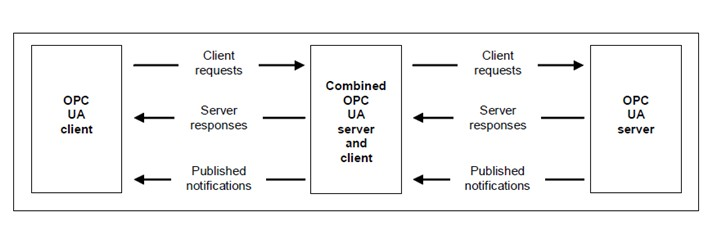
\includegraphics[width=1.00\textwidth]{cs.jpg}
		\caption{OPC UA Client Server Structure\cite{O1}}
	\label{fig:cs}
\end{figure}
Figure~\ref{fig:cs} illustrates a typical OPC UA client server architecture and also describes an internal combined server-client structure. The routine communication between client and server consists of requests from client, corresponding responses sent by server and notifications which are generated because of client's early subscription.

\subsection{OPC UA Terminologies}
In OPC Unified Architecture on server stored information that can be visited by clients is defined as \emph{address space}\cite{O3} and there also exits a set of services\cite{O4} which are provided by server and are introduced in order to apply operations on \emph{address space}. Information in address space is organized as a set of in particular hierarchy structured \emph{Objects}. \emph{Object} here could refer to data gathered by sensor, server system parameters and etc. Clients can query and accept information provided by OPC Unified Architecture Servers in two major ways, \emph{binary structured data} and \emph{XML documents}, depending on the complexity of exchanged data, network quality and so on. In addition three kinds of transport protocol are already defined to support client server communication. They are: \emph{OPC UA TCP}, \emph{HTTP/SOAP} and \emph{HTTP}. Also the hierarchy structure in which \emph{Objects} are organized in \emph{address space} is also various and not only limited to simple single hierarchy.   

One of the charming features provided by OPC UA is \emph{Event Notifications}. With the help of \emph{Event Notification}, OPC UA servers are allowed immediately after satisfaction of conditions, which is normally predefined by a client, to publish data to particular client. In this way, clients can for instance discovery failures within client-server-communication quickly and recover that communication as soon as possible, which in return minimizes the lost to the smallest possible amount. Also clients are able to observe the subscribed data more precisely and find the pink elephant as fast as possible.

\subsection{Standard OPC UA Server}
\begin{figure}[!htbp]
	\centering
	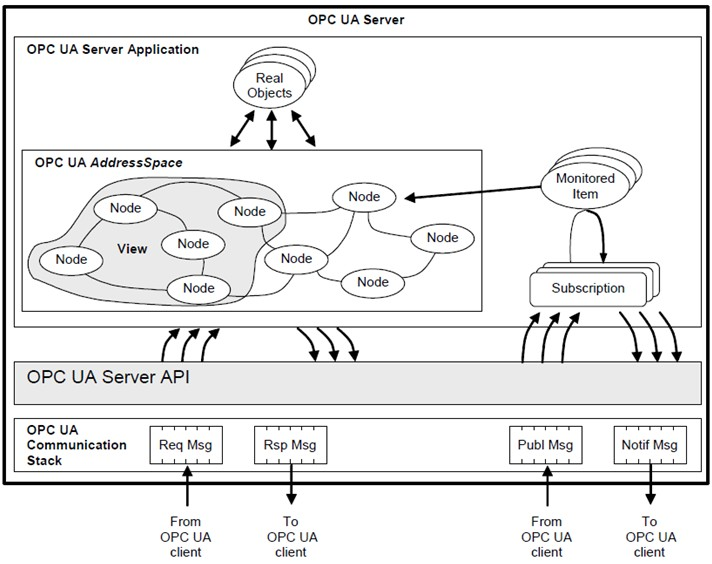
\includegraphics[width=0.8\textwidth]{server.jpg}
		\caption{OPC UA Server Structure\cite{O1}}
	\label{fig:server}
\end{figure}
In figure~\ref{fig:server}, the structure of one standard OPC UA Server is described. It includes three main parts, server application, internal API and communication stack. In server application part,  functionalities and services which are offered by OPC UA standards are realized, such as \emph{Event Notification} , processing request from connected OPC UA client, data encryption and decryption. Moreover, \emph{Real objects}  here  refers physical field devices and software applications that are maintained and managed by OPC UA server. \emph{Nodes} in \emph{Address Space} presents  abstractly above mentioned \emph{Real Ojbects}. \emph{View}, which is pictured as a part of address space, presents \emph{Objects} that can be browsed by particular clients. The main  task for communication stack  is to establish communication session based on secure channel between OPC UA client and server. Typically communication messages which are exchanged frequently among clients and servers are, request-, notification- message from client and   corresponding   response-, publish message from server. At last, an internal API connects the server application and the communication stack.

\subsection{Standard OPC UA Client}
\begin{figure}[!htbp]
	\centering
	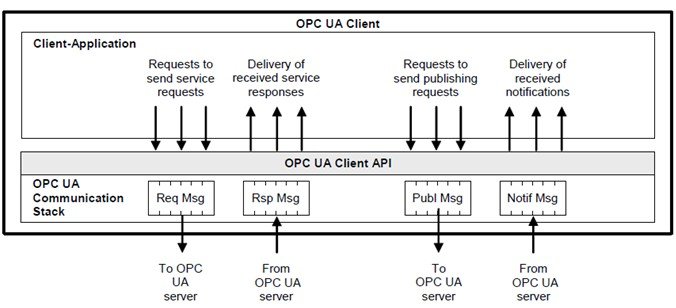
\includegraphics[width=1.0\textwidth]{client.jpg}
		\caption{OPC UA Client Structure\cite{O1}}
	\label{fig:client}
\end{figure}

Figure~\ref{fig:client} pictures one simple OPC UA client containing client application, an internal API, isolating the application code from communication stack, and a communication stack that converts API calls into messages and delivers them to OPC UA server.

\subsection{Secure Channel and Session}

\begin{figure}[!htbp]
	\centering
	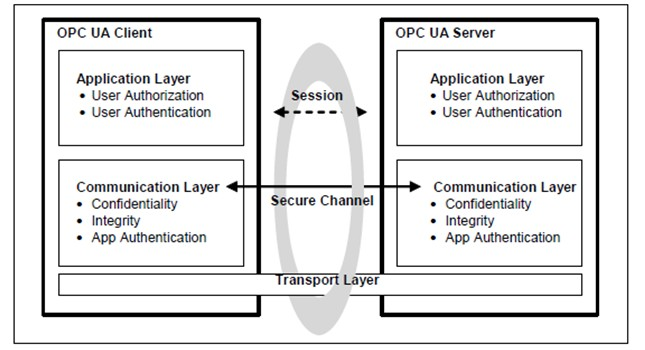
\includegraphics[width=0.8\textwidth]{opc_ua_cs_comm.jpg}
		\caption{OPC UA Client Server Communication\cite{O2}}
	\label{fig:opc_ua_cs_comm}
\end{figure}

Since some data exchanged between client and server could be extreme precious and should be protected from other malicious third party, OPC UA defines a full set of  \emph{security model}, with which sytem developer can configure the security level of the application to meet the need of reality. In the \emph{security model}, authentication of client and server, authorization, integrity and confidentiality of client-server-communication, auditability(also known as traceability ) and availability of services are guaranteed. Also OPC UA  standard provides a set of countermeasures against attacks such as message flooding, eavesdropping, message spoofing, message alteration, message reply, server profiling, session hijacking and so on\cite{O2}.


Figure~\ref{fig:opc_ua_cs_comm} pictures the typical communication architecture between OPC UA client and server. As shown in~\ref{fig:opc_ua_cs_comm}, the communication between OPC UA client and server is established above a secure channel, which is active during the whole application session and in this session, the state information, such as algorithms used for authentication, user credentials, is maintained. The secure channel is established only after successful validation of both client and server certificates and it provides necessary mechanisms to support confidentiality, message integrity and application authentication. On top of secure channel, is an application level session between OPC UA client and server, whose responsibility is to transmit data information and commands. It should be pointed out that, even a secure channel is out of work for some reasons, the session is still valid and OPC UA client and server involved in aforementioned session can still re-establish the broken secure channel. A secure transport layer is guaranteed by encryption and signatures methods provided by platform that supports OPC UA structure.

\begin{figure}[!htbp]
	\centering
	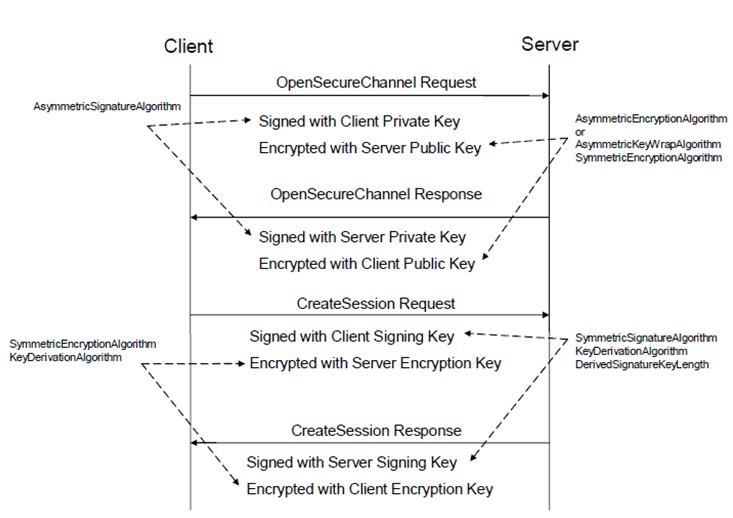
\includegraphics[width=1\textwidth]{opc_ua_shs.jpg}
		\caption{OPC UA Client Server Security Handshake\cite{O2}}
	\label{fig:opc_ua_cs_shs}
\end{figure}

\subsection{Security Handshake}
Security handshake as below explains with some details how secure channel and session are established. Normally OPC UA client initiates the first \emph{OpenSecureChannel} request and waits the response from server. Messages exchanged during the process of construction secure channel between client and server are encrypted using asymmetric encryption and signature algorithms. But some security protocols that could be applied according to OPC UA standards, are not using an asymmetric message encryption algorithm to encrypt to request/response messages. Instead, they apply AsymmetricKeyWrapAlgorithm to encrypt symmetric keys and use symmetric encryption algorithm with encrypted keys to encrypt messages. After a successful construction of secure channel, OPC UA client sends \emph{CreateSession} request and waits for server response. Messages transported during this procedure are encrypted with symmetric encryption algorithms and signed with client/server signing key.
\begin{figure}[!htbp]
	\centering
	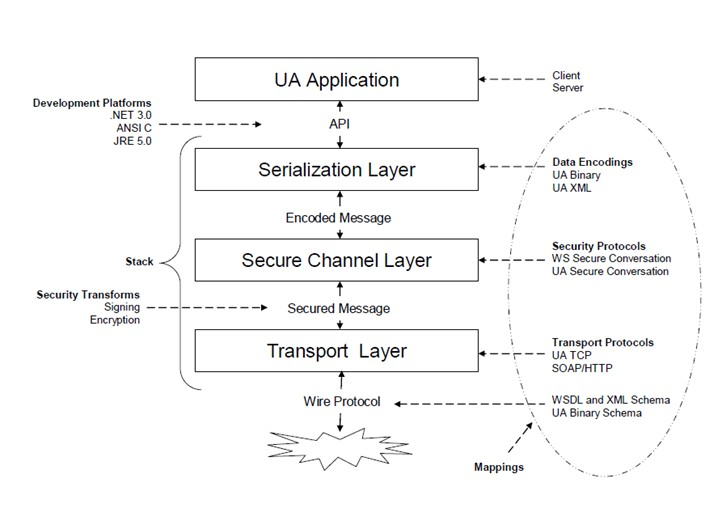
\includegraphics[width=1\textwidth]{opc_ua_commstack.jpg}
		\caption{OPC UA Client Server Communication Stack\cite{O2}}
	\label{fig:opc_ua_commstack}
\end{figure}

\subsection{OPC UA Communication stack}
As described in figure~\ref{fig:opc_ua_commstack}, according to different responsibility, OPC UA communication stack consists of three parts: application layer, communication layer and transport layer. Even the terminologies of those layers using the same English words as the ones used in ISO model, but they are not equal to layers in ISO model. Figure~\ref{fig:opc_ua_commstack} also pictures a precise functionality overview of each component.

UA Application part realizes client or server application. Serialization layer together with secure channel layer build the communication layer and their job is dividing long message into pieces referred as message chunk, encrypting each individual message chunk and forwarding encrypted message chunk to transport layer. When receiving message chunk from others, OPC UA message receiver firstly verifies whether this message piece meets the security standard negotiated between OPC UA client and server. If not, message receiver will close the secure channel. After a successful verification of all message chunks, the original OPC UA message will be reconstructed and sent to UA Application Code through API. Each secure message chunk applies the following structure described in figure~\ref{fig:opc_ua_messchunk}.

\subsection{Other Competitor}
WebSphere Message Broker Message Queuing Telemetry Transport (MQTT)\cite{Ref3} is another machine to machine (M2M) communication protocol. Compared with OPC UA standard, MQTT also supports UDP protocol in the transport layer. In OPC UA, only unidirectional, client to server, communication is provided, but in MQTT server to client communication is also possible without server implements client code. Moreover the communication overhead of MQTT is in comparison with OPC UA is relative small. 


Even thought MQTT protocol supports communication environment with low bandwidth and high latency, OPC UA provides complex object model and supports more features, including historical data record, alarm, notification, complete security policies and this is reason why OPC UA is more suitable for the application scenario that handles sensitive data with complex structure and needs immediate response.


Another member from Internet of Things is Constrained Application Protocol (CoAP)\cite{Ref5} which is designed for the extreme simple electronic devices with less memory and computing power and original CoAP only runs over UDP. Compared with OPC UA, simplicity from CoAP is the advantage, but apparently it should be considered that in the implementation scenario other transport protocol could be used, like TCP, more functions and services other than pure message exchange between client and server, are requested from users.

\section{Smart card}
\subsection{Overview}
Smart Card, whose characteristic feature is an integrated circuit that is embedded in a chip card, which is capable of performing data process, information storage and message transmitting\cite{handbuch}. The most charming feature of smart card is that, sensitive user's credential data such as certificates, encryption keys, digital signature along with other precious user information can only be accessed though a serial interface, which stands under  strict control of the card operation system. This characteristic provides strong  protection against  unauthorized data access and ensures the confidentiality of on card stored information. Therefor smart cards are widely used in applications that require strong protection.

With sophisticated communication protocol using Application Protocol Data Units(APDU), smart card and Card Accepting Device(CAD) are able to process secure message exchange. Smart card is also able to process cryptographic algorithms on hardware. Nowadays, it supports symmetric key algorithms like DES, triple DES; standard public key cryptography for instance RSA, hash functions such as commonly SHA-1\cite{handbuch}. More powerful microprocessor on chip card is, the speed performance is better.  

\begin{table}[ht]
\caption{ISO/IEC 7816\cite{handbuch}}
\centering
\begin{tabular}{lllll}
 ISO7816 document & Description  \\[1ex]
\hline\hline
 ISO 7816-1&Physical characteristics   \\
ISO 7816-2&Dimensions and location of the contacts   \\
 ISO 7816-3& Electronic signals and transmission protocols   \\
ISO 7816-4&Industry commands for interchange  \\
ISO 7816-5& Number system and registration procedure for application identifiers \\
ISO 7816-6& Interindustry data elements  \\
\hline
\end{tabular}
\label{table:ISO7816}
\end{table}

In ISO/IEC 7816 standards family,  the smart card's fundamental properties and functionalities are defined.

\begin{figure}[!htbp]
	\centering
	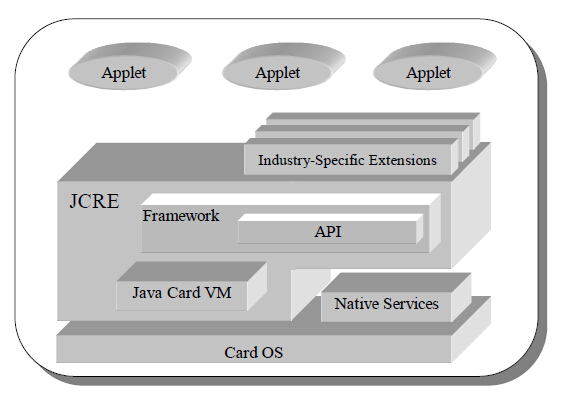
\includegraphics[width=0.8\textwidth]{scc.jpg}
		\caption{Smart Card Software Components\cite{jcadg}}
	\label{fig:scc}
\end{figure}

\subsection{Universal integrated Circuit Card}
The Universal Integrated Circuit Card is the smart card used in mobile terminals in GSM and UMTS networks. It enables authenticated subscriber to join the network with their mobile terminals and at the same time protects essential user data. UICC acts  also most time as the secure token, which stores and protects subscriber's confidential information. Moreover, as a 32bit processor, UICC is also capable of processing necessary  encryption and  decryption algorithms\cite{uiccDef}.

\subsection{Smart Card Software Components}
As illustrated in figure~\ref{fig:scc}, one typical smart card software includes Card Operation System, native services such as I/O operation and memory management, Java Card Runtime Environment(JCRE) that consists of Java card  Virtual Machine and Framework who is in charge of dispatching APDU as well as applet management, installed applet and at last other optional industry specific extensions\cite{jcadg}

\subsection{Smart card File Management}
One of smart card's characteristics is data storage media. But in contrast with other storage device, the most distinguishing feature of smart card file system is that, there exists no man-machine interface\cite{handbuch}, which means all files are addressed with help of hexadecimal codes and every single file process command is strictly based on this shema.

\begin{figure}[!htbp]
	\centering
	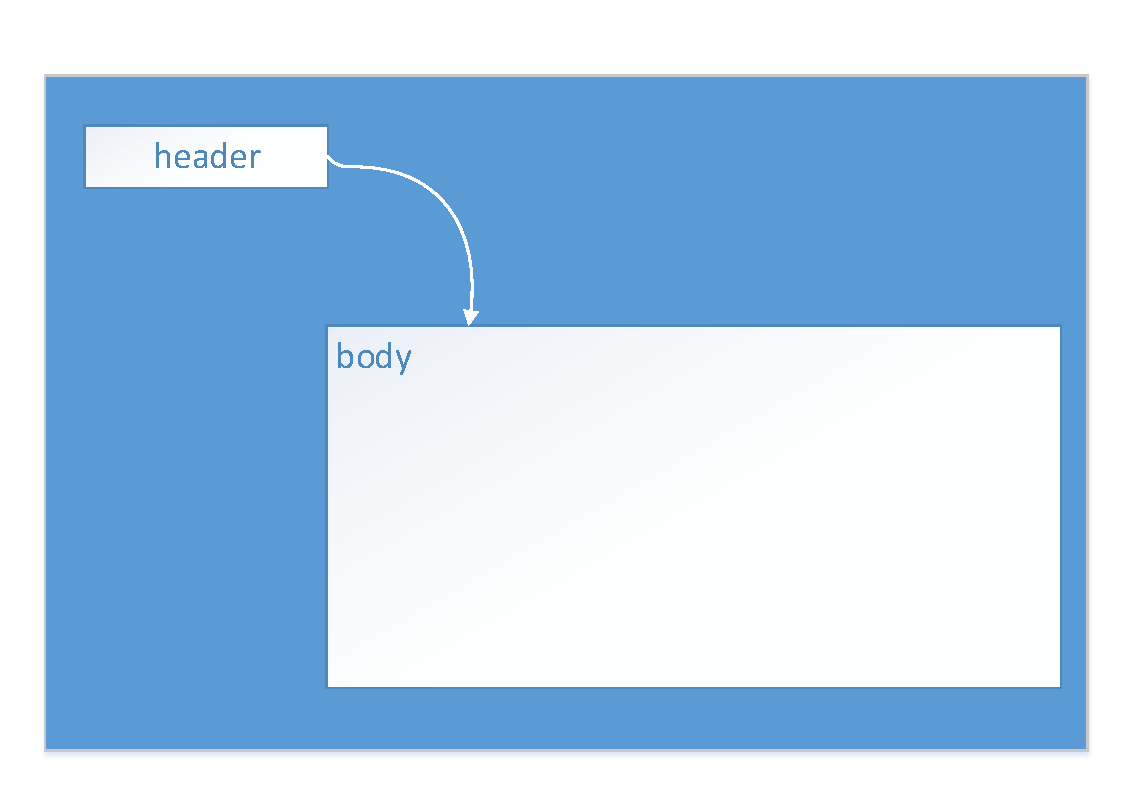
\includegraphics[width=0.8\textwidth]{file}
		\caption{the internal structure of a file in smart card file management system\cite{handbuch}}
	\label{fig:file}
\end{figure}

\subsubsection{File Structure}
As pictured in figure~\ref{fig:file}, files on smart card consist of two parts,  the header, which encapsulates administrative information such as, file structure and access conditions, the body, that stores real user data and is linked with file header using a pointer. This file management mechanism has its own advantage. To be more specifically, since file header and body are separately located, therefore even write/read error occurs in file body, file header, which is under normal circumstances never altered and saves essential access conditions, will not be affected, which in return provides better physical storage security.

\subsubsection{File Types}
According to ISO/IEC 7816-4 specification, smart card offers two major file types, dedicated file (DF) and elementary file (EF). DF is also described as directory file, which contains lower-level DFs and EFs. And in EF, real user data is stored. Moreover there is a special DF, called master file (MF), which represents root directory of smart card file system and only selected by smart card OS. Figure~\ref{fig:file-structure} illustrates one possible architecture of smart card file system.

\begin{figure}[!htbp]
	\centering
	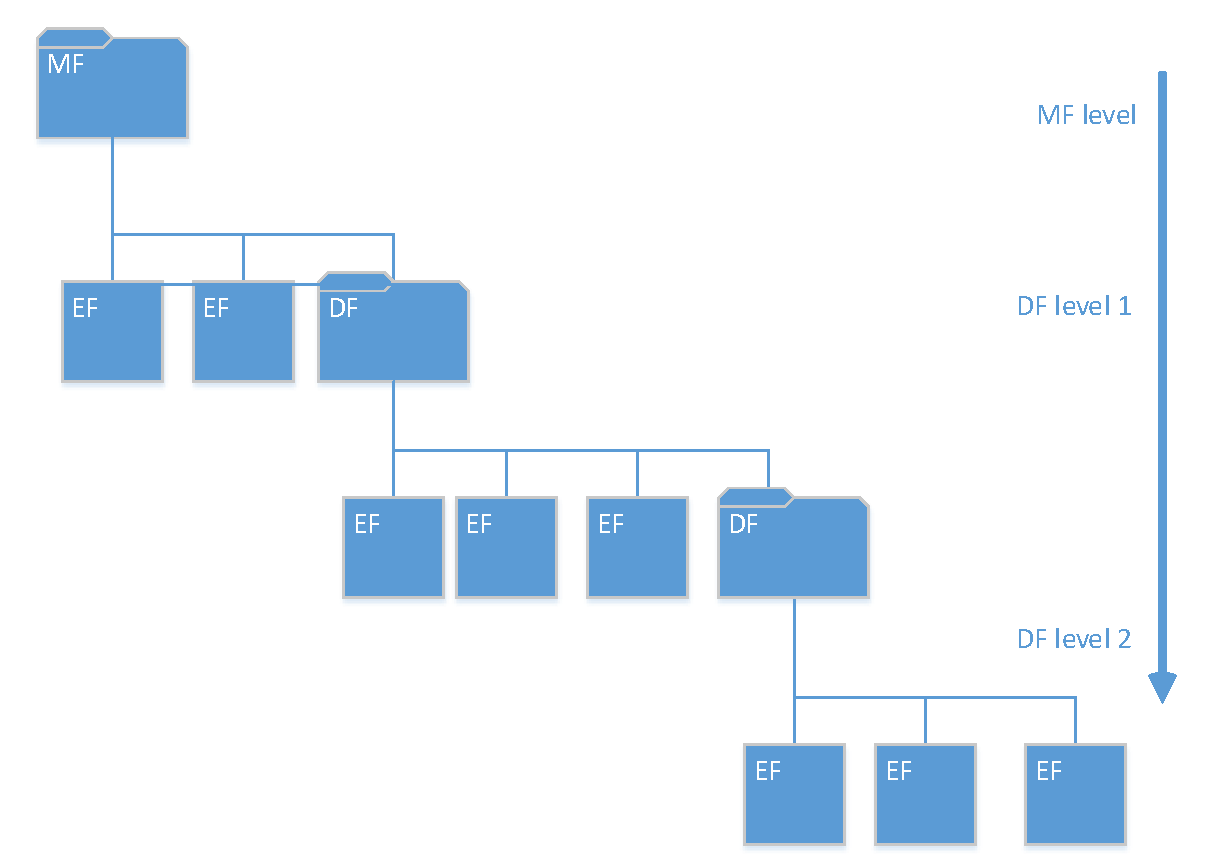
\includegraphics[width=1.0\textwidth]{file-structure}
		\caption{File Tree on Smart Card\cite{handbuch}}
	\label{fig:file-structure}
\end{figure}

\subsubsection{PKCS{\#}15}
As already shown, smart card not only is used as storage media but also acts as cryptographic token which offers enhanced security and privacy functionalities for other applications. The PKCS\#15 (Public key cryptography standards) specification\cite{pkcs}, which was proposed by RSA Inc. and is nowadays worldwide accepted, provide standards, that define how to store credential information such as cryptographic keys, certificates on smart card, and how to retrieve specified token with help from PKCS\#15 interpreter.
 
\subsection{Data Exchange with Smart Card}

\begin{figure}[!htbp]
	\centering
	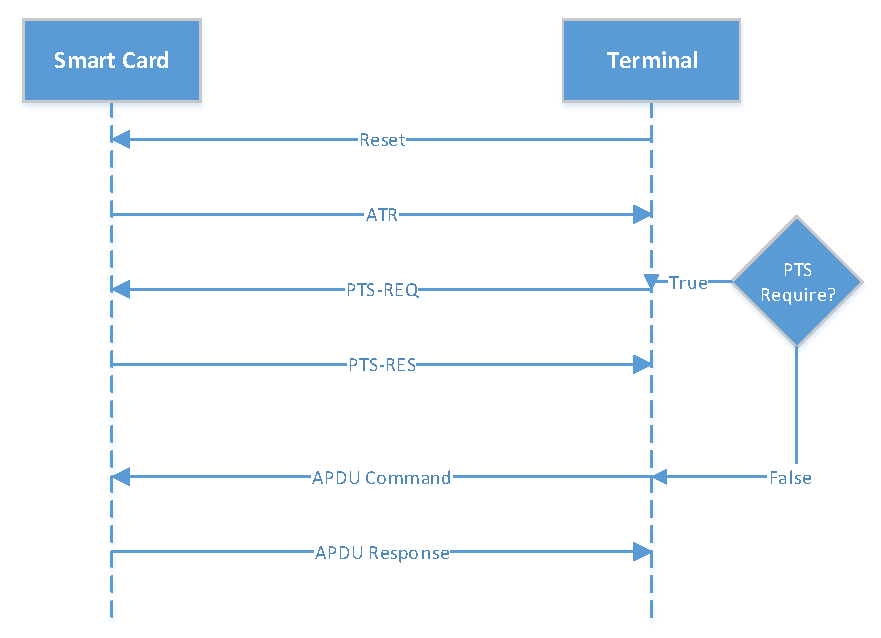
\includegraphics[width=1.0\textwidth]{master-slave-relationship}
		\caption{Communication between Smart card and CAD\cite{handbuch}}
	\label{fig:master-slave-relationship}
\end{figure}
The communication protocol between smart card and terminal is described as Master-Slave relationship\cite{handbuch}, that means terminal device knowns as Master processes unidirectional control over its slave, namely smart card. Once Master-Slave relationship is established, each communication will be initialized by Master and Slave only reacts based on Master's command. 

When a smart card is inserted in a terminal, Master will send its Slave a RESET command which causes smart card to perform a Power-on-Reset behavior. After this Power-on-Reset, smart card informs Master using Answer-to-Rest (ATR) message about card state and communication parameters. In the next step, if necessary terminal will generate a Protocol Type Select (PTS) command, which is used to choose communication protocol and parameters suggested by smart card. After a successful negotiation, smart card and terminal are able to exchange data using Application Protocol Data Unit.
  
Application Protocol Data Unit, or APDU for short, is used  to perform data exchange between smart card and CAD and its structures satisfy ISO 7816-4 specification\cite{chen}. There are two categories of APDU, namely command APDU and response APDU. Command APDU structure and response APDU structure are described in Table~\ref{table:capdu} and Table~\ref{table:rapdu} respectively\cite{handbuch}. 

\begin{table}[!htbp]
\caption{Command APDU Structure}
\centering
\begin{tabular}{lllll}
\hline\hline
 CLA &class byte identifying application  & mandatory \\[0.5ex]
 INS &instruction byte representing the actual command  & mandatory \\
 P1 &parameter 1 used to provide more command information & mandatory \\
 P2 &parameter 2 used to provide more command information& mandatory \\
 Lc field &the length of data received by card & mandatory \\
 data field &data sent to card& optional \\
Le field &the length of data sent by card \\
\hline
\end{tabular}
\label{table:capdu}
\end{table}

\begin{table}[ht]
\caption{Command APDU Structure}
\centering
\begin{tabular}{lllll}
\hline\hline
 data field & length decided by Le of preceding command  APDU  & mandatory \\[0.5ex]
 SW1 &state word 1 also called return code 1  & mandatory \\
 SW2 &state word 2 also called return code 2& mandatory \\
\hline
\end{tabular}
\label{table:rapdu}
\end{table}

\subsection{Secure Messaging}
Since all communication between smart card and terminal is based on digital electrical pulse performed on card I/O line, attacker can easily record all communication information and and recover it. Therefore secure messaging mechanism is proposed and used to protect against aforementioned message eavesdropping, to ensure authenticity and confidentiality of exchanged information.

In secure message mechanism, both message sender and receiver must agree on to be applied message cryptographic algorithms and corresponding pre-shared keys. In telecommunication domain in accordance with ISO/IEC 7816-4\cite{handbuch}, TLV(Type-lengthl-valuse)-formed data, which encapsulates relative user information, is used to perform secure messaging as data carrier.

\section{Java Card}
Java Card technology not only adopts the distinguishing features from Java, such as productivity, security and portability\cite{jcadg}, it also makes Java technology available on smart card, where programmer must be faced with more harsh conditions, like limited memory resource and computer ability.

In contrast with Java VM, Java Card VM consists of two parts, the on-card part, which is in charge of bytecode execution, class as well as object management and secure data exchange, the off-card part, which is the real Java Converter.
 \begin{figure}[!htbp]
	\centering
	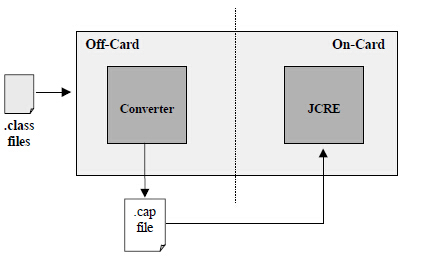
\includegraphics[width=1\textwidth]{jcvm.jpg}
		\caption{Java Card VM Components\cite{jcadg}}
	\label{fig:jcvm}
\end{figure}
As illustrated in figure~\ref{fig:jcvm}, a complied Java applet (.cap file) is generated by off-card Converter based on inputed Java class file and executed by on-card Java Card Runtime Environment (JCRE). 

\subsection{Language Specification}
Apart from above mentioned Java Card VM, compared with original Java language, Java card has many unique features.
Since current smart card does not support multitasking, therefore threads are not backed up in Java Card. Also garbage collection  is performed by VM, as a result function \emph{finalize()} is not supported. Moreover because on smart card, memory space and process ability is limited, as a result programmer can only use three main primitive types, namely byte, short and boolean. Furthermore only one-dimensional array is offered. Nonetheless Java card language supports all features of inheritance and provides all Java language security features, for example, private access modifiers as well as bytecode verification\cite{jcadg}.

\subsection{Transaction Integrity}
One of the most import features of Java Card technology is that Java Card Runtime Environment ensures the integrity of transaction, which means even an unexpected loss of power occurs on smart card, the ongoing transactions' integrity is protected with the help of following schema\cite{handbuch}:
\begin{verbatim}
// Transaction Starts
JCSystem.beginTranscation();

doSomething

//Transaction Ends
JCSystem.commitTransaction();
\end{verbatim}
Only when JCRE finishes running method \emph{JCSystem.commitTranscation()}, the corresponding transaction will be finished and submitted. Otherwise JCRE will throw transaction exception and reset data that involved in this broken transaction.

\subsection{Persistent Object and Transient Object}
In  the realm of Java Card, all objects are preserved in nonvolatile memory, which means this persistent object exits on smart card beyond the execution time of corresponding applet, as long as there exits a reference pointing to it. But also it is allowed to develop transient object on Java card. To be precisely, for instance class array object stays in nonvolatile memory space but in contrast one actual instance of array in stored in volatile memory\cite{handbuch}.

\subsection{Java Card Applet}
Java Card Applet refers to the Java Card language programmed code, which extends the class \emph{Applet} from package \emph{javacard.framework}. Meanwhile Java Card Applet should implement following four methods:
\begin{itemize}
\item\emph{install()}, this method must be implemented and be used to create an applet instance.
\item\emph{process(APDU)}, the implementation of this method is also mandatory and uses APDU as input parameter. In this method applet developer designs how to process APDU sent to this applet and which APDU response should be generated.
\item \emph{select()}, when JCRE detects a SELECT APDU command, which is applied to select one installed applet, JCRE will call this method of to be selected applet.
\item  \emph{deselect()}, this method is called by JCRE to inform corresponding applet that it is no longer selected by JCRE.
\end{itemize}

\begin{figure}[!htbp]
	\centering
	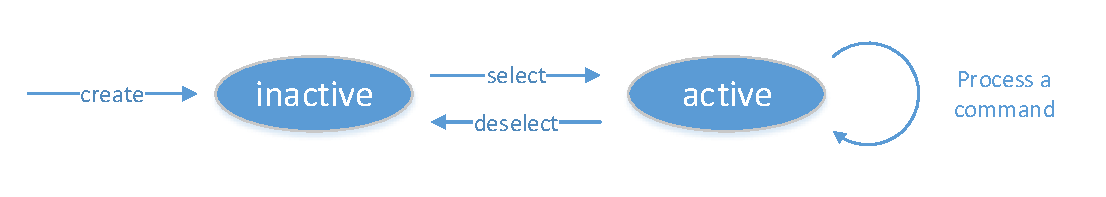
\includegraphics[width=1\textwidth]{applet-execution-states}
		\caption{Javacard Applet Execution States\cite{handbuch}}
	\label{fig:applet-execution-states}
\end{figure}
After finishing programming one Applet, it comes to next phase, namely applet installation. This process takes place usually at the factory or office under the control of card issuer. When one applet is installed on smart card, it only directly communicates with JCRE and other installed applet classes. It should be pointed out, this installed Java Card applet is also belongs to \emph{persistent object} and stored in smart card nonvolatile memory space. Every Java Card Applet is assigned one unique Application ID, which is also known as AID and be used by JCRE to \emph{register} and \emph{select} corresponding applet at run time.

Figure~\ref{fig:applet-execution-states} pictures execution states transaction of Javacard applet. Furthermore figure~\ref{fig:apdu-command-processing} illustrates how JCRE selects and deselects one applet based on input APDU commands.

\begin{figure}[!htbp]
	\centering
	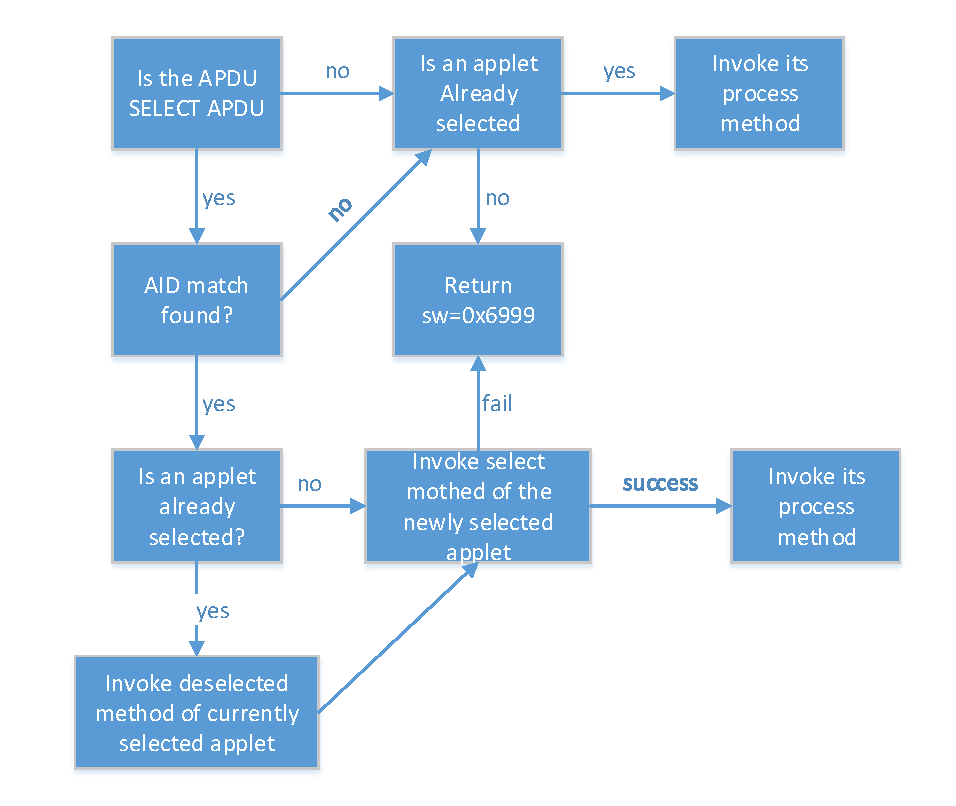
\includegraphics[width=0.8\textwidth]{apdu-command-processing}
		\caption{APDU command processing\cite{handbuch}}
	\label{fig:apdu-command-processing}
\end{figure}


\subsection{Javacard Cryptography}
Javacard provides a list of APIs to support not only smart card application and data exchange security but also to reinforce other system's security by acting as essential security token. 
In order to ensure sure messaging between smart card and terminal following three aspects must be considered:
\begin{itemize}
\item \emph{Entity Authentication:} Usually mutual authentication is applied to guarantee the authorities of both communication partners.
\item \emph{Message Confidentiality:} The transfered information is encrypted using algorithms negotiated between two communication entities to ensure data privacy and security.
\item \emph{Message Integrity:} In order to protect exchanged message from unauthorized modification and to provide authenticity assurance, message authentication code (MAC) is calculated based on to be transfered data and integrated in that message.
\end{itemize}
Packages \emph{javacard.security} and \emph{javacardx.crypto} support aforementioned security mechanism with following class and interfaces\cite{chen}:

\begin{table}[ht]
\caption{package: \emph{javacardx.crypto}}
\centering
\begin{tabular}{lllll}
\hline
 Class or Interface & Function Description\\
\hline\hline
Cipher & Abstract class offers cryptographic cipher used for encryption and decryption\\
KeyEncryption & Class provides implementation of keys\\
\hline
\end{tabular}
\label{table:javacardx-crypto}
\end{table}

\begin{table}[ht]
\caption{package: \emph{javacard.security}}
\centering
\begin{tabular}{lllll}
\hline
 Class or Interface & Function Description\\
\hline\hline
 Key &Interface for all keys   \\
 SecrectKey &Interface for symmetric algorithms' keys\\
DESKey & Interface for keys used for DES or two-key triple DES or three-key triple DES\\
PrivateKey &Interface for private keys\\
PublicKey & Interface for public keys\\
RSAPrivateKey& Interface for keys used by RSA algorithm to sign data\\
RSAPublicKey & Interface for keys used to verify signatures generated with RSA \\
DSAKey& Interface for keys used by DSA\\ 
DSAPrivateKey& Interface for keys to sign data with DSA algorithm\\
DSAPublicKey& Interface for keys to verify signatures generated with DSA\\
KeyBuilder& Factory class implemented to construct key objects\\
MessageDigest& Abstract class for hashing algorithm\\
Signature& Abstract class for signature algorithm\\
RandomData&Abstract class for generation of random data \\
CrptoException& Exception class\\
\hline
\end{tabular}
\label{table:javacard-security}
\end{table}


\section{GlobalPlatform and Remote Application Management}

\begin{figure}[!htbp]
	\centering
	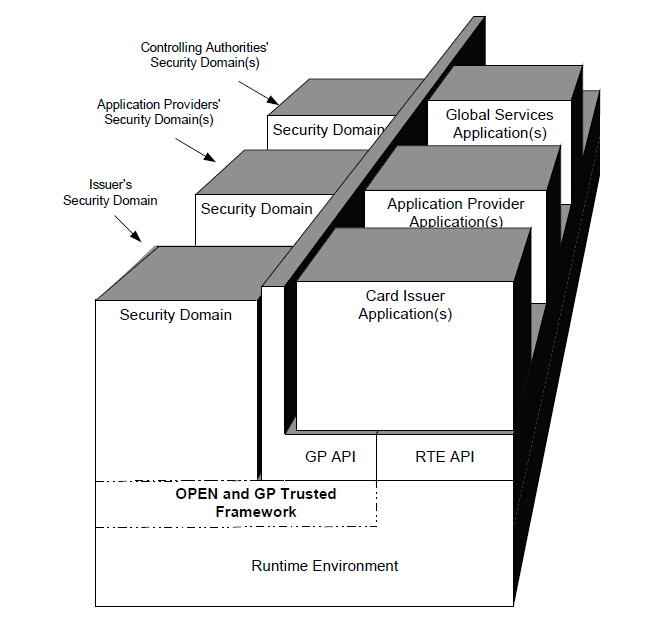
\includegraphics[width=0.7\textwidth]{gp_1.jpg}
		\caption{Card Operation System Architecture\cite{gp}}
	\label{fig:gp_1}
\end{figure}
GlobalPlatform is an international non-profit organization that provides standardized specifications for multiple smart card applications. It is now widely accepted and used as industry standard for managing Java Applet based application on Javacard Operation System in several domains, for instance in communication industries and payment company\cite{gp}. 

As shown in figure~\ref{fig:gp_1},  the GlobalPlatform card architecture contains four essential parts. The runtime environment, that provides hardware-neutral API for card application  and manages card memory spaces. The on card installed applications, which offers customers various functionalities and services. The security domain (SD), that is usually associated with particular application and known as on-card representatives  of off-card  authorities. SD is in charge of message encryption as well as decryption, creation and validation of digital signature and handling keys used in cryptographic processes. The last component is OPEN framework\cite{gp}.

\subsection{OPEN - GlobalPlatform Environment}
OPEN provides various sets of APIs offering functionalities such as entity authentication, remote data exchange, secure channel configuration and remote application management. This framework also performs APDU dispatching as well as is application selection and logical channel management\cite{gp}. Logical channel is designed to enable the data exchange between multi applications and one terminal. Each opened logical channel will handle message regard of one application.  Moreover the special logic channel named basic channel is always opened. In order to ensure system security, OPEN supports secure mechanisms such as,  user authentication , resource availability guarantee and secure channel protocol .
\paragraph{Secure Channel Protocol}
In particular, GlobalPlatform has designed the secure mechanism: secure channel protocol, to guarantee a secure communication. It ensures confidentiality of exchanged information and offers data integrity check.  Moreover Secure Channel Protocol also introduces  a cryptographic exchange process to let smart card and off-card entities to perform entity authentication with each other. 
 \begin{figure}[!htbp]
	\centering
	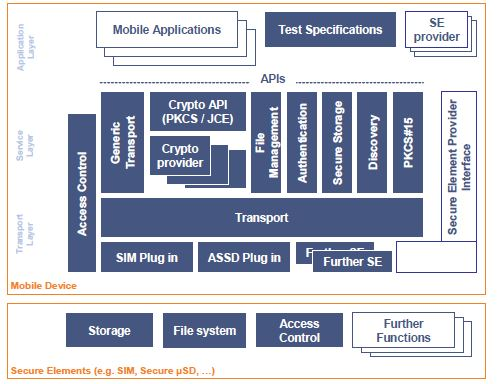
\includegraphics[width=0.8\textwidth]{open-architecture.jpg}
		\caption{OpenMobileAPI architecture overview\cite{open}}
	\label{fig:open-architecture}
\end{figure}

\section{OpenMobileAPI}
OpenMobileAPI, provided by SIMalliance, constructs an interface between terminal and chip card, which can be used by on terminal installed mobile application to access recourse stored on smart card as well as call function provided by smart card applet. Moreover OpenMobileAPI offers security mechanisms such as access control, that can be applied for mutual authentication between application and secure element. Figure~\ref{fig:open-architecture} presents an architecture overview of OpenMobileAPI, which consist of three functional layers:
 \begin{itemize}
  \item \emph{Transport Layer:} This layer is in charge of providing secure elements access control services using APDUs and acts as cornerstone for other two layers.
  \item \emph{Service Layer:} Abstract interfaces, that provide various functions such as secure storage, cryptographic services, are offered by this layer.
  \item \emph{Application Layer:} Mobile applications which benefit from OpenMobileAPI lie in this layer.
\end{itemize}

\section{Android}
\subsection{Overview}
Android is an open source platform based on Linux and modified by Google, which is designed for mobile devices. As a comprehensive platform, android manages to create a separation between hardware and software that runs on it.  At the same time being an open source platform means its entire stack is open and android developer are able to deploy their androids on specific hardwares as well as to learn the system to the fundamental level.\cite{learn_android}
Moreover, android system provides a list of software and hardware attracting features to his customers.
 \begin{itemize}
\item \emph{Security:} Linux, as the cornerstone of android, has been proved to be a secure system through many harsh tests over the years. Which in return guarantees the android system security. \cite{learn_android}
\item \emph{Multi-Media:} A wide range of media formats are supported by Android. For instance: MPEG4, ACC, PNG, GIF and so on. \cite{android_media} Which in return provides android users a more comfortable user experiences and better entertainment functionalities.
\item \emph{Designed for Online:} One outstanding core feature of Android system is the ability to stay Online\cite{android_forensics}. Under various conditions such as Wi-Fi network, GSM/CDMA and so on, android device always provide its end users qualified network connection.
\item \emph{Variety of applications :}As one of the most popular platform,  Android, with the help of Android Market and great number of talent Android application developers, offers its customers the ability to extend  functionalities of their android devices\cite{android_forensics}. Android user is capable of downloading and installing various innovative applications from Android Market and enhancing the user experience.
\end{itemize}
\subsection{Android Software Stack}
\begin{figure}[!htbp]
	\centering
	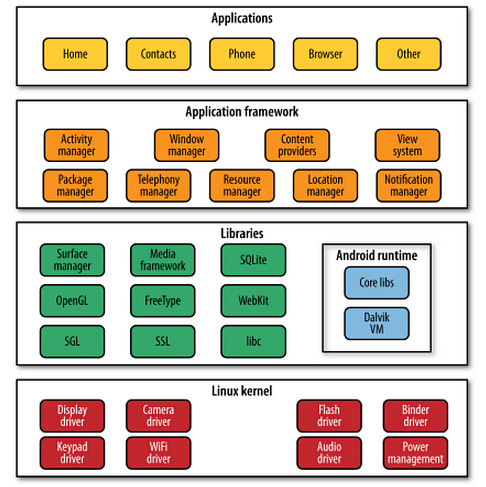
\includegraphics[width=1.0\textwidth]{android-stack.jpg}
		\caption{Android Stack Overview \cite{learn_android}}
	\label{fig:android-stack}
\end{figure}
Android stack is composed of four different layers as shown in figure~\ref{fig:android-stack}.

\subsubsection{Linux kernel:}This fundamental layer separates other three layers  from  device hardware and provides higher layer core  functions such as  power and hardware driver management.
\subsubsection{Libraries:}As second layer of android stack,  Libraries layer supports android runtime environment by applying various C/C++ core libs, that offer most of the Java-functionalities.  Also in this layer, the for android specific designed virtual machine, namely Dalvik\cite{learn_android} is deployed. There exits two reasons for not using standard Java VM\cite{learn_android}. First of all, since Java VM is general developed virtual machine, therefore some constrains from mobile systems and devices are not concerned, such as limited battery life and processing ability. Secondly, when android project  was being carried out,  Java VM didn't  belong  to the open source projects. For these reasons Dan Bornstein and his group developed the license free and mobile platform specific virtual machine, Dalvik. 

Apart form  android runtime, other libraries which provide services to application framework layers are also included in this Libraries layer, for instance:
\begin{itemize}
\item OpenGL, library that supports 2D and 3D graphics rendering.
\item SSL, the widely applied secure socket layer library.
\item  SQLite, which provides lightweight SQL database services.
\item  WebKit, the fast  web-rending engine.
\end{itemize}
\subsubsection{Application  framework} Application framework layer provides a large amount of application framework components, for instance activity manager which is in charge off managing application life cycles, content providers that controls data exchange between applications.
\subsubsection{Application}As the top layer of entire android software stack, application layer with the help of both native and third party reside component from application framework layer, provides various services to end users.

\section{Android, Dalvik and Java}
As described above, Dalvik VM compared with general Java virtual machine, takes the constrains that are specific about mobile device into account, which means this android virtual machine concerns the hardware shortcomings including less memory space, low processing power, no swap space as well as short battery lifetime. Minimum recommendations for android device\cite{android_vm} are list in table~\ref{android-min-req}.
\begin{center} 
\begin{table}[h]
\caption{Minimum Android Recommendations\cite{android_vm}}
\label{android-min-req}
\begin{tabular}{|l|l|}
\hline
Feature          & Minimum Requirement                                                                                                   \\ \hline
Chipset          & ARM-based                                                                                                             \\ \hline
Memory           & 128 MB RAM; 256 Flash External                                                                                        \\ \hline
Storage          & Mini or Micro SD                                                                                                      \\ \hline
Primary Display  & QVGA TFT LCD or larger, 16-bit color or better                                                                        \\ \hline
Navigation  keys & \begin{tabular}[c]{@{}l@{}}5-way navigation with 5 application keys, power,\\ camera and volume controls\end{tabular} \\ \hline
Camera           & 2MP CMOS                                                                                                              \\ \hline
USB              & Standard mini-B USB interface                                                                                         \\ \hline
Bluetooth        & 1.2 or 2,0                                                                                                            \\ \hline
\end{tabular}
\end{table}
\end{center}

 \begin{figure}[!htbp]
	\centering
	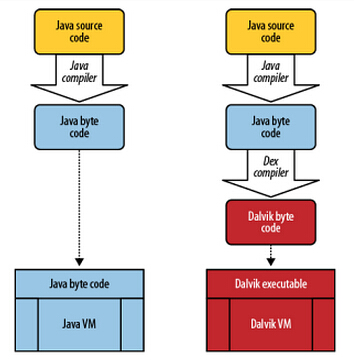
\includegraphics[width=0.7\textwidth]{vm-compare.jpg}
		\caption{Compiling process difference\cite{learn_android}}
	\label{fig:vm-compare}
\end{figure}
When Dalvik virtual machine is applied, the compiling process is different from what is taken by Java VM. Figure~\ref{fig:vm-compare} clearly pictures the difference. In Android runtime environment, after the first compilation of Java source code, the newly generated Java byte code will be compiled by Dalvik Dex complier, as a result, Dalvik byte code is created, which is going to be executed by Dalvik VM.

As pictured in figure~\ref{fig:class-vs-dex}, compared with \emph{.class} Java byte code, \emph{.dex} code adopts shared and type specific constant pools with the main purpose of conserving memory\cite{android_vm}. To be more specifically,  the constant pool in Java byte code, which is colored blue in left side of above-mentioned figure, is heterogeneous, which means all kinds of constant pools are included in this heterogeneous constant pool, even if they could be unnecessary. As a consequence, duplication may occur in Java byte code.    

Another obvious distinguish between Java VM and Delvik is that, the former one adopts stack-based architecture and  the later one uses register-based architecture, that in comparison with stack-based architecture needs on average 32.3\% less execution time\cite{android_vm}, which is obviously the better choice for the system that runs on mobile devices with limited battery life.

 \begin{figure}[!htbp]
	\centering
	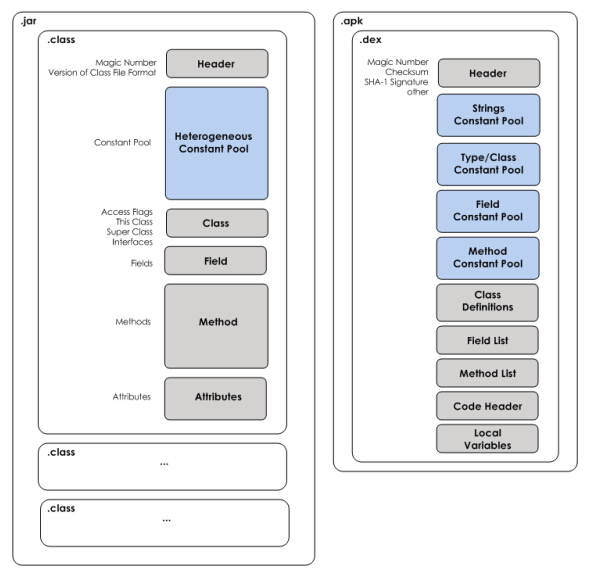
\includegraphics[width=1.0\textwidth]{clas-vs-dex.jpg}
		\caption{Comparison between Java byte code and Dalvik executable file\cite{android_vm}}
	\label{fig:class-vs-dex}
\end{figure}

\clearemptydoublepage
\chapter{State of Art}
In this chapter, I firstly discussed the current researches in the realm of home automation system, in order to achieve inspiration materials for my demonstration scenario. Also after studying the industrial smart home application cases listed in this thesis, I have concluded that present-day automation systems commonly require a well-defined communication interface among all the housing devices, system as well as information security is still strongly demanded, which in return proves that my proposal is meaningful and promising.  

The second topic covered by this chapter is the study of security. In more details, I have studied security   technologies and mechanisms employed in OPC UA standards as well as Smart Card system and Android applications. With the acknowledgment of aforementioned studies, I have learned the potential threads to my application system as well as how to provide corresponding countermeasures. Moreover, in the last paragraph, I introduced  the general guild-line for the development of a secure embedded system, which enlightened me about how to design my demonstration system.
 
\section{Smart Home Research}
\subsection{Overview}
The smart home system, which is also described as automated home, integrated home system or intelligent building \cite{smart_home_concept}, has drawn more and more industry developers' and researchers' attention over the decades. Research groups from for instance Siemens, IBM, Cisco, Microsoft has already contributed in this domain \cite{smart_home_research}. A great number of Smart Home applications, network protocols as well as gateways have come into world and been applied to benefit their customers \cite{smart_home_for_gateway}.

With the development of Smart Home technology, nowadays' Smart Home not only is in charge of monitoring and controlling lighting and heating devices inside the building, but also capable of connecting almost every electronic housing devices, predicting inhabitant behavior as well as making scheduler decisions. Functionalities provided by intelligent home are not just limited to turn device on and off, record and report senor data, but include self-adjusting the inner building environment and supporting various predefined patterns, such as energy saving pattern. Especially the concept of Smart Home for elderly \cite{smart_home_for_old}, which perfectly combines modern remote control and monitoring technologies with senior-friendly and patient-concerning housing techniques, is welcomed by the market. 

Three categories of Smart Home will be introduced in the following as best practice examples, they are Smart Home optimized for energy services , Smart Health Home and Agent-based Smart Home.
 
\subsection{Smart Home Optimized for Energy Services}
This type of Smart Home sets its main goal in the energy saving and monitoring domain, which helps householder to make wiser decisions under the energy crisis background. 

The key component in this Smart Home is decision-support tool \cite{smart_home_for_energy}, that applies a scheduling algorithm which offers house owner energy saving suggestions based on various variables such as distributed energy resources (DER), with the prospect of saving precious energy and resource.

\subsubsection{Decision Support Tool}

 \begin{figure}[!htbp]
	\centering
	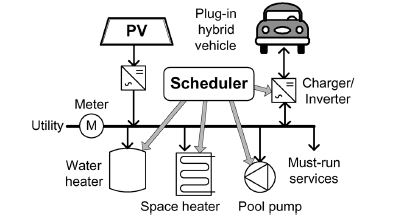
\includegraphics[width=1.0\textwidth]{scheduler.jpg}
		\caption{DER Scheduler in Smart Home optimized for energy\cite{smart_home_for_energy}}
	\label{fig:smart-home-scheduler}
\end{figure}

The decision support tool used in paper \cite{smart_home_for_energy} consists of two components, they are energy service model which describes the energy service request and distributed energy resource scheduling algorithm, as described in figure~\ref{fig:smart-home-scheduler}. To be more specifically, energy service model presents the demand of one particular energy resource. For instance the demand aimed at hot water means, the hourly consumption of heated water or the energy that is hourly needed by water heater.  According to paper \cite{smart_home_for_energy}, the heat content of water is also defined as "energy equivalent" and therefore the main goal of decision support tool is to increase "monetary benefit"  from every "energy equivalent" unit.

The DER scheduler algorithm, that helps householder to reduce the unnecessary consumption of energy, is in nature one mathematical optimization problem defined as following \cite{smart_home_for_energy}.
\begin{center}
 $ \sum_{t=1}^{T}\sum_{i=1}^{S}[\lambda_{ES,i}(t)\cdot {U_{ES,i}}(t,x)]-Cost$
\end{center}

The purpose of DER scheduler presented as \emph{x} is, to maximize that above introduced fitness function, where \emph{S} represents all number of services offered by Smart Home, \emph{T} stands for the whole simulation time, $\lambda_{ES,i}$ and $ U_{ES,i}$ describe the desired monetary benefit for "energy equivalent" and energy demand of the \emph{i}th service respectively. \emph{Cost} means the total electricity consumption. Also in paper \cite{smart_home_for_energy} the choice of DER algorithm is well discussed.


\subsection{Smart Health Home}
Another suitable application domain for Smart Home is the Smart Health Home, which describes the intelligent housing that takes care of patients and elder residents.

The charming feature of this Smart Home system is the combination of home automation technologies with telemedical system, which provides customized services such as, teleconsulting, telediagnosis, real time imaging as well as long distance medical education \cite{smart_home_for_health}. Smart Health Home will improve the living condition of householder and at the same time build a concerning system that takes care of residents' need. Nine best practice examples are provided and evaluated in paper \cite{smart_home_for_old}, they provide a guide-line for the design of Smart Health Home system and summarizes precious experience. 
 \begin{figure}[!htbp]
	\centering
	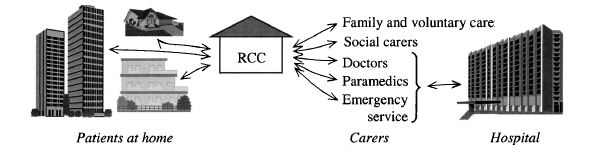
\includegraphics[width=1.0\textwidth]{rcc.jpg}
		\caption{Overview of Smart Health Home structure \cite{smart_home_for_health} (RCC: Remote Control Center)}
	\label{fig:rcc}
\end{figure}
\subsection{Agent-based Smart Home} \label{secAgent}
Agent-based Smart Home aims to build an intelligent home, which is based on machine learning, artificial intelligence technology and mobile computing. The core features of agent-based Smart Home are, prediction of householders' behaviors and making appropriate decisions. The achieved prediction can help residents to experience a more comfortable and convenient living condition. MavHome (Managing An Intelligent Versatile Home) builds the best demonstrating example \cite{smart_home_agent} . 

\subsubsection{MavHome Architecture}
 \begin{figure}[!htbp]
	\centering
	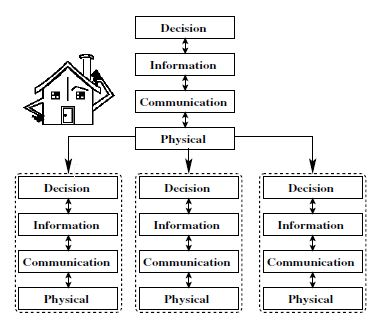
\includegraphics[width=0.8\textwidth]{smart-home-agent.jpg}
		\caption{MavHome agent architecture \cite{smart_home_agent}}
	\label{fig:smart-home-agent}
\end{figure}
As shown in figure~\ref{fig:smart-home-agent}, agents which are employed by MavHome consist of four different layers. From bottom to top:
\begin{itemize}
\item \emph{Physical layer}, where Smart Home system device hardwares are deployed. Moreover, underlaying agents can also act as physical layer for other high level agents.
\item \emph{Communication layer}, this layer provides communication service for agent by using functionalities offered by physical layer.
\item \emph{Information layer}, as higher layer of Smart Home system,  the responsibilities of this layers are gathering and maintaining information which is going to be required by decision layer.
\item \emph{Decision layer}, in this layer agents make decision as well as learn resident's preference. Moreover, with the help provided by learning algorithms, agent is also able to correct the unwanted system behavior and learn from bad decisions.
\end{itemize}
\subsubsection{Prediction Algorithm}
Prediction algorithm is the core component of MavHome project. several strategies are presented on the first IEEE international conference on pervasive computes and communication, they are SHIP algorithm that is based on sequence matching, compression-based prediction algorithm ALZ and Task-based Markov model \cite{smart_home_agent}.

\subsection{Conclusion}
As described above, Smart Home is the representative application which is based on industrial automation, remote management and coordination system. Despite the decision making algorithms and application level components from above mentioned smart buildings are different from the other, but they all are integrated upon or connected with housing devices. The management and cooperation with those devices must take place under a secure system environment. None of householders are willing to be monitored by a strange third party using his own camera or to expose their daily life related information to the public. Therefore one common request for the design of such intelligent buildings is to ensure the system security.

Based on the fact, that home devices applied by Smart Home are manufactured by various vendors,  Smart Home designers also must take it into account, that how to realize the system interoperability. Considered those two requirements, the proposal of this thesis is proved as practical and desired.

\section{OPC UA Application and Security Policy}

\subsection{OPC UA Applications}
OPC UA, as explained in former paragraphs,  is understood as a platform independent, well designed, security concerning, IEC standard compliant, promising industry standards set, which provides a service oriented architecture and is being widely applied in industry fields such as critical control system and industrial automation. Application cases are given in following paragraphs, each of them has different focuses. To be more specifically, the charming demonstrated characteristics of OPU UA applications are: strong security protection, real time data exchange as well as coordination and scalability. 

\subsubsection{OPC UA and ICS}
With the development of industrial automation technology, Industrial Control System (ICS) has became a hot topic, but most manufactures invested much more effort in designing automation as well as manufacturing process and neglected the communication security issues. As a consequence, cyber security of ICS is now drawing more and more attentions. OPC UA offers manufacturers who are applying ICS system not only sophisticated object oriented modeling rules, which can be extremely helpful for developers to design domain specific model and manufacturing process, but also provides them a reliable and robust security model \cite{opc_ics}, that has various secure arrangements in each layer of software architecture.


\subsubsection{OPC UA and Smart Grid}
Smart Grid is now considered as the future of electricity energy industry and therefor how to design an intelligent electricity distribution system, which coordinates the customer-supplier relation, becomes the most popular topic \cite{opc_grid}. Electricity industry is searching out for a standardized communication and connectivity technology to solve aforementioned issue.
OPC UA standards set that includes \emph{alarm and even} model, \emph{data access} model as well as  \emph{historical data access} model, is without doubt one the of best candidates. With the help of all aforementioned models, the secure real-time peer communication and coordination among stockholders are guaranteed.

\subsubsection{Nano OPC UA }
Apart from those enterprise level systems, OPC UA is also suitable for lower level field devices, such as field sensor and other resource limited facilities. Recently a German company Lemgo even designed a nano embedded OPC UA server \cite{opc_lemgo}, which provides the core OPC UA server service set. adopts TCP binary communication protocol and is implemented on a chip device.

\subsection{OPC UA Secure Policy}
At the beginning of OPC UA standards design phase, the OPC foundation has taken the construction of a secure and robust communication protocol as the center of their work and therefore developed an enhanced consistent security model which has clear and definite objectives in each layer of OPC UA software architecture. At the present day, OPC UA  offers secure messaging mechanisms by applying WS security with Simple Object Access Protocol (SOAP)  and alternatively SSL based Hypertext transfer Protocol Secure (Https) messaging \cite{opc_secure_1}. Besides secure messaging protocols,  authentication mechanisms based on username-password or X.509 certificates are also introduced, in order to perform mutual authentication among OPC UA applications from different logic levels and hardware devices.

OPC foundation introduces the term \emph{secure policies} \cite{O2} to describe the 
user authentication, user authorization, application authentication as well as message encryption mechanisms proposed by one OPC UA server profile. In this server profile, both secure related requirements and other server functionalities are described. One server is capable of maintaining several profiles in order to provide distinguishing services to different clients, who might have various security demands. Meanwhile one client can also accept a list of profiles, each of them is assigned by a different server. 

\subsection{OPC UA Secure Consideration}
Along with core services set including data read and write operations, notification mechanism and etc, OPC UA server also provides the \emph{discover service} \cite{O4}, which provides OPC UA clients the mechanism to require server secure policy. Moreover a \emph{secure channel service} set \cite{O4} is also designed, which is use to create and manage secure channel with the acknowledgment such as key deviation algorithm and message encryption algorithm, that are described by a secure policy. 

Also OPC UA specifications provide guide lines for a secure system design \cite{O4}. They are:

\begin{itemize}
\item \emph{appropriate timeout}. Timeout mechanism is widely employed in systems that adopt client-server architecture. With reasonable configured timeout property, both client and server can avoid unnecessary resource consumption caused by long time waiting of response from the other, which could be the consequence of an unexpected physical device failure or denial of service attack, which is intentionally initiated by an adversary.
\item \emph{Message exchange rate control}. Rate control is considered as one of the most practical approach to prevent denial of service attack. Under rate control mechanism, each client has limited chance over a period to build communication channel, reconstruct this channel, require information from server or send data to server. Alternatively the OPC UA server can also ban or block a client for a period of time, who was recently trying to flood messages. 
\item \emph{random number generation}. The generation of random number is required by most encryption, authentication and authorization algorithms. Therefore a secure system must support and provide a robust random number generation function.
\item \emph{strict message processing}, which means the exchanged message between two communication partners must be compliant with predefined message format. Any ill-formed messages must be ignored, which in turn helps to avoid stack overflow attack and enhances system security
\item \emph{historical data management}, this strategy ensures the system traceability and records any behaviors taking place in system. The recorded data can be used for forensic research, when security related issue happens.
\end{itemize}
\subsection{Conclusion}
Above pictured OPC UA standards' features and characteristics prove the feasibility of applying OPC UA as communication protocol for Smart Home proposed in this thesis and the study of industrial application cases helps me to present this point better.

\section{Smart Card Security}
Integrated Circuit Card, ICC for short, was firstly designed and patented in Germany \cite{smart_card_history}. Since then this credit sized, embedded with circuit chip card is being applied in a great number of industry domains working as for instance information storage media, on-line access token, identification method, small amount payment mechanism and etc. With the development of smart card technologies, nowadays apart from traditional \emph{contact smart card}, \emph{contactless smart card} \cite{smart_card_contactless} has come into the market. This \emph{contactless smart card} is able to communicate with card accepting device without direct physical connection. To be more precisely, it applies radio frequency to contact with CADs. Now matter what categories of smart card, the tamper resistant nature always contributes to make them to be the most popular secure token media.
\subsection{Smart Card in Access Control Management}\label{secSCAC}
The present-day concept of \emph{security} no longer just meant the secure of our homeland borders or the individual personal safety. In this information age, the word \emph{security} also refers to the confidentiality and integrity of users' personal data, the robustness of information system and so on. It is immediately related with our daily life. Especially when electronic devices, which can carry sensitive as well as precious information and could be vulnerable to malicious attackers, are playing irreplaceable roles in our society. 

Smart card, as explained in section \emph{fundamental technologies}, is believed as one of the best secure mechanism for access control and user identification. 

Traditionally there are three ways to identity a person \cite{handbuch}:
\begin{itemize}
\item \emph{1 knowledge about a secret}, the secret is normally a password that negotiated earlier between two identification peers.
\item \emph{2 possession of an object}, this object could be anything that is predefined. One example could be the key that can open a particular door.
\item \emph{3 biometrics identification}. First two approaches have their own limitations, because third part could steal the object, that is used for identification, or copy user's password. Moreover it also could happen, that a password is too complex to remember or identification object is difficult to carry with. Compared with them, biometrics identification  however depends on the unique human body characteristics, such as fingerprint and retina recognition.
\end{itemize}
Based on the above described facts, smart card is the best candidate for user identification and access control. Because when anyone wants to perform identification using smart card, he must possess the card (possession of an object satisfied), input PIN to unlock the card (knowledge about a secret). At the same time, complex passwords for the purpose of peer authentication and authorization can be stored on the smart card, which helps card holder to release the burden of remembering them. Also on a chip name card, which is usually carried by a card-holder in order to access a secured room or building, there usually exists a signature signed by the card-holder or his photo, that could be use to perform biometrics identification. 

Nowadays with the help of standards such as \emph{remote application management} protocol, which is introduced in \emph{fundamental technologies} section~\ref{secGP}, smart card is also capable of performing on-line identification based on either certificate or TLS protocol.

\subsubsection{Personal Identification Number}
Whenever an user intends to use one smart card, he must input a \emph{personal Identification Number}, which is also referred as \emph{Card Holder Verification}. PIN consists usually of four decimal number from 0 to 9 and tolerates at most 3 times wrong PIN input before a successful verification. PIN is stored in elementary files  \cite{smart_card_access} on smart card, in order to be protected from unauthorized modification. After 3 times wrong PIN input, a smart card will be locked until the \emph{unlock PIN} operation is successfully performed. Moreover if \emph{unlock PIN} operation also fails three times in a roll, the PIN will never be unblocked \cite{smart_card_access}.

\subsection{Smart Card Key Management Mechanism} \label{labelKeyManagement}

 \begin{figure}[!htb]
	\centering
	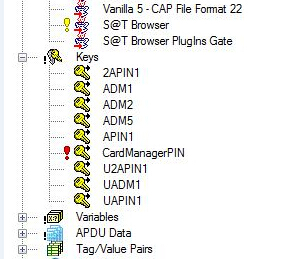
\includegraphics[width=0.5\textwidth]{smart-card-key.jpg}
		\caption{Keys Presented in Smart Card Description Language Developed by \emph{Morpho}}
	\label{fig:smart-card-key}
\end{figure}

The above introduce PIN is not the only key that is stored on the smart card. In order to perform message encryption as well as decryption, peer authentication and etc. smart card must keep various keys in storage. As shown in figure~\ref{fig:smart-card-key}, in a \emph{Morpho} smart card product, a list of keys and key sets are designed such as Card Manager PIN and Administrative keys (\emph{ADM1, ADM2, ADM5}).

Moreover, the key data stored on a  smart card records not only the actual key value but also provides information such as key version number and the usage of key as shown in Table~\ref{table:smart-card-key}. Likely, in order to retrieve the value of a key from smart card, user must provide information such as key identifier and key version as shown in figure~\ref{fig:smart-card-key-use}.

 \begin{figure}[!htb]
	\centering
	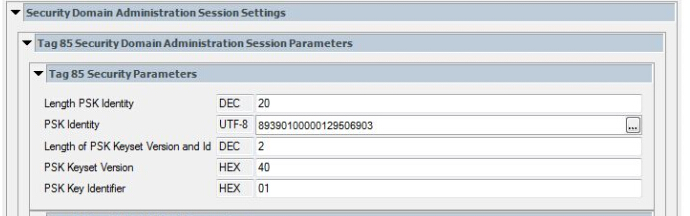
\includegraphics[width=0.85\textwidth]{smart-card-key-use.jpg}
		\caption{the PSK Key Used to Configure Administration Session}
	\label{fig:smart-card-key-use}
\end{figure}

\begin{table}[!htb]
\caption{Key Data Stored in Smart Card\cite{handbook}}
\begin{tabular}{lllll}
\hline\hline
Data object & Remarks\\[0.5ex]
Key number & unique key reference number\\
Version number & version number used for key derivation\\
Intended usage & for which purpose this key is introduced\\
Blocked & used to block a key\\
Retry counter & wrong key input counter\\
Maximum retry count & key will be blocked if retry counter reaches this value\\
Key size & the size of key\\
Key & Key value\\
\hline
\end{tabular}
\label{table:smart-card-key}
\end{table}

Since different keys play distinguishing roles in various system tasks and smart card must handle a huge number of keys, \emph{key management} mechanism shows its importance. The core responsibilities of smart card key management system are listed as following \cite{handbook}:
\begin{itemize}
\item \emph{key generation.} Key generation is the initial step of key life cycles and uses usually physical random numbers as initial data, in order to generate secure and unique keys. 
\item \emph{key update.} This process keeps one key from being used for a long period of time. Because long time service of one key could lead to the compromise of system security.
\item \emph{key revocation.} When one key turns out to be compromised, key management system must destruct that key.
\item \emph{key storage.} Apparently a competent key management system must know how to safely store its secrets.
\end{itemize}
\subsubsection{Key Generation}
\paragraph{Derived Key}
Since smart card can be easily exposed and analyzed by anyone who holds or steals the card, in order to minimize the risk of key compromising, none master keys are present in the smart card. As a consequence, keys used in smart card are derived from unique card number, which is given during the card production phase, with the help of triple DES and AES cryptographic algorithms \cite{handbook}.
\paragraph{Dynamic Key}
Dynamic key is normally applied to protect communication between peers and therefore it is also known as the session key or temporary key. The generation of dynamic keys begins with the generation of a random number that is proposed by one communication partner or unique data which is able to specify one particular session. There is a number of dynamic key generation approaches and I will take \emph{ANSI X 9.17} standard as an example \cite{handbook}. 
\begin{center}
$Key_{i+1} = e(Key_{gen},e(Key_{gen},(T_{i} XOR Key_{i})))$
\end{center}
The function described above is one-way process and can not be reserved. To be more specifically, $T_{i}$ and  $Key_{gen}$ are the time as well as session independent initialization input parameter and Key generation key respectively. The newly generated  key $key_{i}$ can not only be used for encryption but also to generate other new keys.
\subsection{Threatens and Countermeasures}
In this section, potential smart card vulnerabilities, threatens aimed at chip card as well as countermeasures will be discussed. But before I present the analysis of smart card threatens, the trust environment of smart card based system should be explained. Following five parties are involved \cite{smart_card_attack1}.
\begin{itemize}
\item \emph{Cardholder.} In other word, the owner of smart card, who daily applies smart card for different purposes in various systems. For instance, using SIM card in cell phone to make phone call or using smart card digital wallet to perform smart amount payment like paying the parking fee.
\item \emph{Terminal.} Terminal is the card accepting device that communicates with smart card through smart card I/O.
\item \emph{Card Manufacturer.} As the name indicates, card manufacturer is the one who manufactures  the card.
\item \emph{Card Issuer.} Card Issuer is the party that designs the card OS and initializes the smart card. For example, if we are taking about a cell phone smart card, then card issuer will be the cell phone service provider. When it comes to employees' ID cards which are applied as access control tool for a company. Then in this situation, the card issuer is the employer.
\item \emph{Software manufacturer.} This party is the one who designs applications that run on smart card.
\end{itemize}
\subsubsection{Threatens and Vulnerabilities}
Since threat modeling for smart card could be extreme complex and also the classification of smart card is various. In this paragraph four representative threaten categories are presented. They are,
\begin{itemize}
\item Logical attacks. Whenever we develop a software, there could exist a bug/bugs. And logical attacks just refer to the attacks that make use of bugs in software implementation \cite{smart_card_attack2}. Two examples are given as follow:
\begin{itemize}
\item \emph{Hidden Commands}. This kind of attack attempts to abuse commands from \emph{initialization phase} of smart card life cycle, to modify or retrieve sensitive data from smart card in poorly designed smart card system. The abused command should have been inactive but not in above mentioned vulnerable system \cite{smart_card_attack2}.
\item \emph{Malicious Applets}. Malicisou applet is a Ill-designed smart card software, that attempts to break smart card system and steal information.
\end{itemize}
\item Physical attacks. This type of attack aims  at reverse engineering data and functions that are contained on smart card. Normally expensive and modern lab equipments are required \cite{smart_card_attack2}. Also physical attack is known as \emph{invasive attack} \cite{smart_card_attack3}. Three kinds of physical attacks are introduced as following :
\begin{itemize} 
\item \emph{Micro-probe station}. Using Micro-probes, adversaries try to construct electrical connection with smart card chip, in order to observer communication between process and memory. With the observed information, attacker is capable of capture sensitive data such as key information and etc \cite{smart_card_attack3}.
\item \emph{Focused Ion Beam}. Also it is possible to transmit intentionally generated signals to smart card processor using focused ion beam. As a consequence, it is possible for attacker to reveal data from smart card \cite{smart_card_attack3}.
\item \emph{Chemical Solvents, Etching and Staining Materials}. Using aforementioned chemical materials, attacker can observe etching speed difference from some ROM memories and with a step further analyze \emph{0} and \emph{1} in those memories \cite{smart_card_attack2}.
\end{itemize}
 \begin{figure}[!htbp]
	\centering
	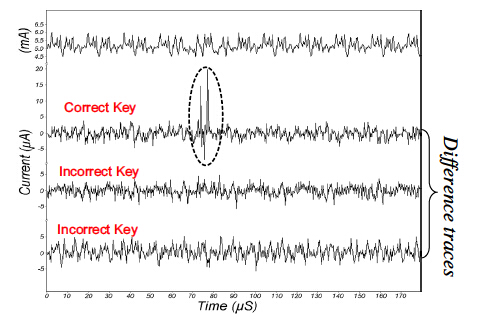
\includegraphics[width=0.8\textwidth]{pda-attack.jpg}
		\caption{Differential Power Attack on a DES implementation \cite{embedded_secure}}
	\label{fig:pad-attack}
\end{figure}
\item Non-invasive attacks. This kind of attack makes use of smart card runtime environments such as difference in power consumption, processor voltage, clock frequency and etc. to analyze smart card behaviors. For example,
\begin{itemize}
\item Power consumption attacks. The execution of smart card operations relays on power provided by terminal.  When attacker is able to observe smart card power consumption, which is used by card performing cryptographic algorithms, he may retrieve related keys by applying \emph{Differential Power attack} or \emph{Single Power attack} \cite{smart_card_attack3}. Figure~\ref{fig:pad-attack} pictures a differential power attack analysis on a DES implementation.
\item Timing attack on RSA. The computing duration of RSA algorithm depends also on the input key. Therefore there is an opportunity for attacker using observed time gap in key computation process to get secret key information \cite{smart_card_history}
\end{itemize}
\item Other Attacks\cite{smart_card_attack5}.
\begin{itemize}
\item Denial of service. This kind of attack aims at impacting smart card performance and consuming smart card system recourses to harm the availability of smart card service .
\item Eavesdropping. Through eavesdropping exchanged information is catapulted and analyzed.
\item Cover transaction. Fake session or session hijacking. Those approaches try to forge a communication session between smart card and the other connection peer, in order to gain information, which is related with peer authentication, authorization and messaging.
\end{itemize}
\end{itemize}

\subsubsection{Countermeasures} \label{secSMD}
\paragraph{Logical Attacks Countermeasure}
In oder to prevent this category of attacks, the number of bugs in smart card application should be minimized. Smart card software developer and card manufacturers can apply \emph{structure design} by dividing application into small units which are easy to be tested and understood. Alternatively companies related in smart card industry should work together to propose standardized interfaces and protocols to regulate the smart card application development process \cite{smart_card_attack2}.
\paragraph{Physical Attacks Countermeasure}
Smart card manufacturers have already realized the potential  invasive attacks and are enhancing the physical security of smart card by offering:
\begin{itemize}
\item Reducing chip size. Now the size of smart card internal components can reach 150 nm, which makes it significantly hard for attacker to perform physical attack \cite{smart_card_attack3}.
\item Metalization layers, which prevent smart card from atmospheric effects \cite{smart_card_attack3}.
\item Multi-layered chips. Smart card manufacturers are now able to build chip card consisting of multi-layers. Vulnerable components, for instance ROM memory, are deployed in the lowest layer and protected from physical analysis \cite{smart_card_attack3}. 
\item Sensors.  Smart card is protected by sensors covered with resin and those sensors will disable smart card whenever they detect physical attacks \cite{smart_card_attack}.
\end{itemize}
\paragraph{Non-invasive Attacks Countermeasure}
Countermeasures against above described non-invasive attack are:
\begin{itemize}
\item Against Timing Attacks by computing \emph{superfluous calculations}, in this way adversaries are not able  to get correct timing gap anymore \cite{smart_card_attack3} .
\item Against Power Consumption Attacks by applying digital noise. Alternatively chip	 manufacturers can reduce the electromagnetic emissions to make power consumption analysis  harder\cite{smart_card_attack3}.
\end{itemize}
\paragraph{Other Attacks Countermeasure}
Other attacks are normal computer security issues and can be avoided by for instance applying message encryption mechanism, building communication session based on secure channel, introducing message transmitting rate control policies and defining appropriate timeout counts.
\subsection{Smart Card Secure Applications}
As given above, smart card is considered as a secure data storage media and a superior tool to protect information system security. People also describes smart card as the \emph{magic bullet}, that can solve computer security issues, such as access control management, peer identification and so on. Understandably, more and more smart cards are applied in secure applications and products. For instance:
\begin{itemize}
\item In Payment System. Recently the concept of electronic purses and electronic payment systems becomes more and more popular. Not only because this newly proposed mean of payment can play a supporting role for traditional payment methods such as credit card, but also because with the integration of smart card, electronic purses are able to offer flexible, reliable and secure small amount payment  services \cite{handbook}.
\item For Peer Identification. Based on the knowledge from section~\ref{secSCAC}, Smart card holder is  capable of performing two factor authentication \cite{smart_card_history}, which requires that at least two of three listed conditions are satisfied. Therefore smart card are suitable for the domain of personal identification. Since December 1999, Finland has begun to use electronic personal ID cards to replace traditional passports \cite{handbook}. 
\end{itemize}
\subsection{Conclusion}
In conclusion, the above discussed security features of smart cards, such as sophisticated key management system and counter measures against potential threads, prove the feasibility and reliability of my proposal, that is applying smart card for secure credential management and adding additional protection for the system which adapts smart card. Moreover with the help of industrial standardized protocols which are introduced in section~\ref{secGP}, card holder can enjoy a secure remote management service and trust the electronic devices which are integrated with smart cards, let those facilities administer his properties.  

\section{Secure Android Design}
With the development of smart phone market, more and more subscribers are using this new generation of cell phones with their smart cards. Accordingly an increasing number of attacks aiming at smart phone platforms is reported. 

 \begin{figure}[!htb]
	\centering
	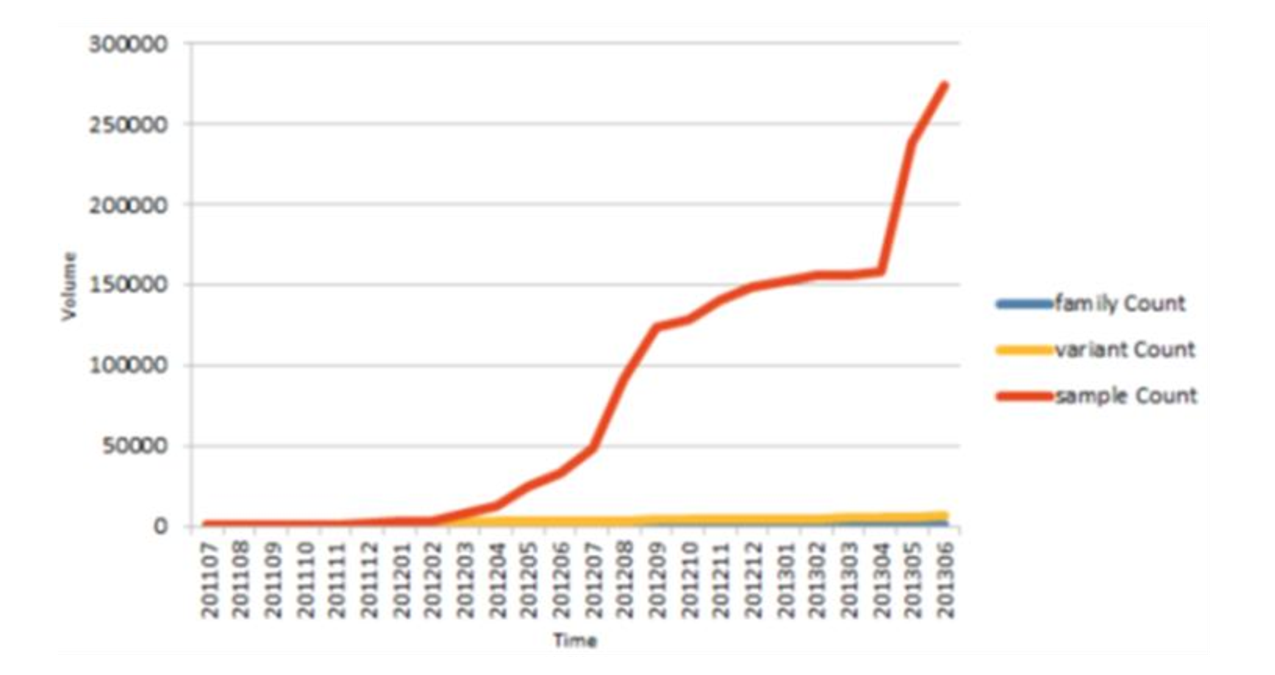
\includegraphics[width=1.0\textwidth]{malware1.pdf}
		\caption{Android Malware Growth \cite{malware}}
	\label{fig:android-malware}
\end{figure}

Figure~\ref{fig:android-malware} shows a dramatic increasing amount of Malwares that target at Android platform from report \cite{malware}. Especially when taken it into account that present-day smart phones are also in charge of sensitive users' information such as recent visited location as well as contacts list.  And based on a study of Android applications, researchers have found that over 20\% applications could have access to user personal data \cite{android_secure_design}. Consequently there exists a pressing requirement for Android application developers to design their Android software with strong security protection. 

\subsection{Android Security Mechanism}
Even though a huge number of third party applications exist on Android market and they could be potential Malwares, but Android platform is not vulnerable and it provides secure as well as robust security mechanisms to protect its customers. Following listed three methods are the most outstanding and efficient approaches.
\begin{itemize}
\item \emph{Application Isolation.} Each Android application has its own Linux process and each of this process possesses an isolated virtual machine. In this way, application data is separated and protected from the other \cite{android_secure_language}. 
\item \emph{Access Permissions.} Permissions are given during the applications' installation time. As illustrated in figure~\ref{fig:android-permission}, Android permission system restricts the access right to user's private data, to other Android applications , to smart phone hardwares and to Android OS. 
\begin{figure}[!htb]
	\centering
	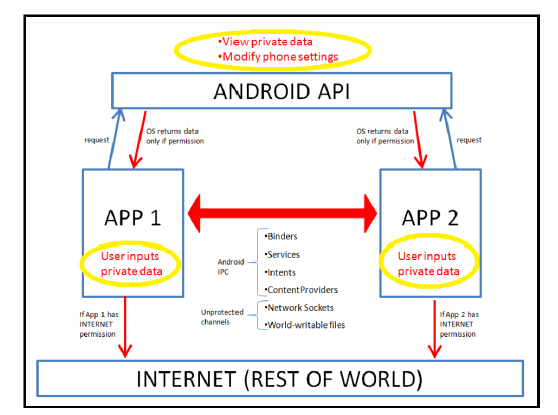
\includegraphics[width=0.9\textwidth]{android-permission.jpg}
		\caption{Detailed Android Permission Model \cite{android_secure_design}}
	\label{fig:android-permission}
\end{figure}
\item \emph{Authorized Signatures.} Applications are signed with certificates. The corresponding private keys are protected only by the application developer. Every time when one application claims his identity, his signatures will be checked, in order to prevent the potential masquerade attacks \cite{android_secure_language}.
\end{itemize}

\subsection{Security Design Guide-Lines}
With the acknowledgment from previous paragraphs, it can be concluded that Android system is designed with consideration of security, especially in the domain of access control and permission management. But still ill-developed application is vulnerable. For instance, when an application carelessly sends an intent introduced in section~\ref{secIntent}, which has none explicit target. This implicit intent can be intercepted by a Malware. As a result, this malicious application may manage to access the sensitive data of victim application and perform attacks such as \emph{activity hijacking} and \emph{service hijacking} \cite{android_secure_inter}.

Therefore it it necessary for application developers to apply protection techniques  in oder to protect their application from attackers and revers engineering. In the following, three secure Android design guide lines are summarized.

\subsubsection{Application Components Secure}
In order to restrict the number of applications, which have access rights to the Android application components described in subsection~\ref{secAppComponents}. Android application designer  should explicitly claim the access control policies in \emph{AndroidManifest.xml} from their project. In extreme case that none applications are expected to invoke the secured component, following rule should be added in \emph{AndroidManifest.xml} \cite{android_secure_cook}.
\begin{Verbatim}[fontsize=\relsize{-1},frame=lines,framesep=4mm, label=\fbox{\small\emph{Component Securing}}]
<[component name] android:exported='false'>
</[component name]>
\end{Verbatim} 

\begin{figure}[!htb]
	\centering
	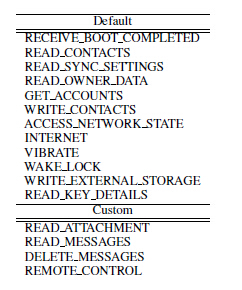
\includegraphics[width=0.4\textwidth]{android-permission2.jpg}
		\caption{Permission Required by Application \emph{k9mail} \cite{android_secure_design}}
	\label{fig:android-permission2}
\end{figure}
\subsubsection{Custom Permissions for Access Control}

As pictured in figure~\ref{fig:android-permission2}, Android OS provides a list of default permissions, which serve a generic access control management, including such as  phone  holder data reading and writing, Internet access right and etc. But when it comes to the case of sharing data between different applications, a more sophisticated and robust custom permission is desired. To be more specifically, following xml snippets, which declare customized permission rules, should be added to the protected components in project's \emph{AndroidManifest.xml} \cite{android_secure_cook}.

\begin{Verbatim}[fontsize=\relsize{-1},frame=lines,framesep=4mm, label=\fbox{\small\emph{Custom Permission Snippet}}]
<permission android:name='android.permission.CUSTOM_PERMISSION'
	android:protectionLevel ='dangerous'
	android:description = 'Custom Permission Snippet'
	android:label = '@string/custom_permission_label''>
\end{Verbatim} 
Moreover four categories of protection level are supported \cite{android_secure_cook}:
\begin{itemize}
\item \emph{normal.} This is the lowest level of permission and usually applied for non-dangerous permissions. 
\item \emph{dangerous.}  In this kind of permission, there exist the risks that authorized application would be able to access user credential information and sensitive data.
\item \emph{signature.} Signature permission means that applications which are signed with the same certificate can access each other.
\item \emph{signatureOrSystem.} In addition to \emph{signature} level, this level of permission will be also automatically granted to the application that is part of system image.
\end{itemize}
\subsubsection{Securing Content Provider}
Last secure approach that I want to present is the content provider path  secure mechanism. Since content provider handles mostly the exchanged data between applications, therefor it frequently becomes the first victim of a system attack. Application developer must ensure the security of content provider, especially the content provider path, which is in nature an uniform recourse identifier that is related  to sensitive information such as datasets \cite{android_secure_cook}. Content provide path may look like \emph{content://com.provider.android/account/balance}.

It is highly recommended that application developer explicitly defines the permission rules at path level, one demonstration example is given as following \cite{android_secure_cook}, 
\begin{Verbatim}[fontsize=\relsize{-1},frame=lines,framesep=4mm, label=\fbox{\small\emph{Content Path Securing}}]
<provider ...>
<grant-uri-permission android:path = 'path_name'>
</provider>
\end{Verbatim} 
\subsection{Conclusion}
In conclusion, Android is  a secure platform with sophisticated access control mechanisms and other security polices. But still Android application developers should apply security techniques to protect their project from malicious and ill-formed applications. Moreover I developed my Android application \emph{Smart Home App} following the above presented Android secure design guide lines. The concrete design and implementation details will be presented in chapter \emph{System Design}. 

\section{Embedded System Secure Design} \label{secESSD}
\subsection{Overview}
In this last section of this chapter, a generic guide for the embedded system secure design is introduced. As already in previous sections described, low level components that build the embedded system compared with traditional  computer software have additional security requirement. For instance, low end devices are normally dependent on battery as electricity supplement and have limited computing capacities. Those two constrains must be taken into account during the design phase of a secure embedded system.
\subsection{Embedded System Security Requirements} \label{5}
The \emph{Trinity of Trouble} \cite{embedded_secure} three factors, namely \emph{complexity},\emph{extensibility} and \emph{connectivity} contribute together to make the embedded system more vulnerable and complicate the system security requirement.
In the following a brief discussion about embedded system security requirements and corresponding solutions are presented \cite{embedded_secure}.
\begin{itemize}
\item \emph{User Authentication}. Before the embedded system performs any functionalities, the identity of system user must be confirmed. Alternatively the user also has the need to verity the embedded system's identity. The expected mutual authentication can be realized by applying secure protocol such as \emph{TLS 1.2} or using digital certificates and signatures.
\item \emph{Content Security}. The security of exchanged message also plays an import roll in a secure embedded system. Message integrity and confidentiality must be ensured. Popular solutions are to apply cryptographic algorithms such as symmetric ciphers, asymmetric ciphers and hash algorithms to protect system content from illegitimate modification and eavesdropping.
\item \emph{Secure Network Connection}. Most devices nowadays have the access to the Internet. As a consequence, secure  network connection belongs also to the security domain in embedded system. In order  to provide a secure network environment, system developer should apply secure communication protocols such as SSL or create secure VPN connection \cite{embedded_secure}.
\item \emph{Secure Storage}. System data must be protected from unauthorized modification and stealing by malicious entities. Therefore tamper resistance hardware should be applied.
\item \emph{Availability}. At last the service availability must be guaranteed by apply anti-DoS attack mechanisms, which are already introduced in this thesis.
\end{itemize}
\subsection{Software Security during Software Design Life Cycle}
\begin{figure}[!htb]
	\centering
	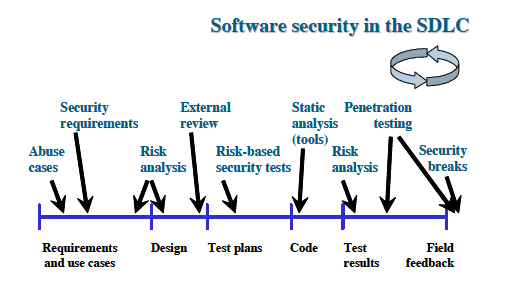
\includegraphics[width=0.95\textwidth]{sdlc.jpg}
		\caption{Software Security Consideration in the Software  Design Life  Cycle \cite{embedded_secure}}
	\label{fig:sdlc}
\end{figure}
With the acknowledgment of system security requirements as well as corresponding solutions, embedded system designer should concern potential security threads as well as system imperfections in each application design phase and perform corresponding security analysis as well as run secure-related tests, as shown in figure~\ref{fig:sdlc}.

\subsection{Secure Architectures}
In oder to keep an embedded system from malicious parities' attacks, especially when present-day system is normally exposed in a ubiquitous networking and pervasive computing environment \cite{embedded_secure}. System developer should design a robust and secure system architecture with the security consideration from architectural micro level to macro level. Figure~\ref{fig:design-space} pictures the choice of architectural design space.\footnote{ASIC:application-specific instruction set processor. EP: embedded general-purpose process. SPx: special purpose extensions. GPx:general purpose extensions. HWaccel: hardware accelerators. GOP: co-processor}
\begin{figure}[htb]
	\centering
	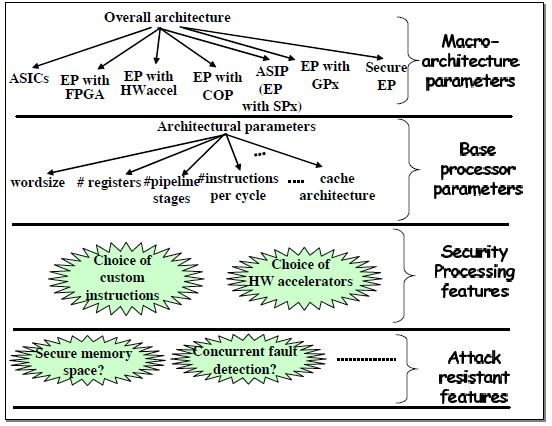
\includegraphics[width=0.9\textwidth]{design-space.jpg}
		\caption{Architectural Design for a Secure Information Processing \cite{embedded_secure}}
	\label{fig:design-space}
\end{figure}

When the hardware architecture characteristics of an embedded system are confirmed. Following two secure aspect as shown in last two rows of figure~\ref{fig:design-space} should be considered
\begin{itemize}
\item \emph{Security Processing Features.} Various fundamental secure protocols and algorithms could be selected by system designer. But some of them may offer the same security services. Therefore in this layer, the choice of cryptographic algorithms should be made with the consideration of hardware and software specific aspect. For instance, the full implementation of SSL protocol for a simple low end filed device is apparently not a wise decision \cite{embedded_secure}.
\item \emph{Attack Resistant Features.} When general security mechanisms used to ensure content confidentiality, data integrity and peer authentication are provided by an embedded system, security mechanisms to prevent other kinds of security attacks such as denial of service attack also should be designed.
\end{itemize}

\section{Conclusion}
In this chapter, I presented industrial application cases in the realm of home automation, OPC UA specifications and smart card products. At the same time, I emphasized the importance and significance of security in those applications. Moreover, I summarized the security mechanisms employed by smart card and OPC UA applications. A generic developer guide line for secure Android application design as well secure embedded system development is provided. Especially, based on the concept presented in section~\ref{secESSD}, before the development of my application system, I have firstly analyzed the security requirements in my scenario and set clear security objectives in each layer of my system components. The five in section~\ref{5} mentioned security requirements are satisfied in my system. The \emph{user authentication} is protected by the PIN as well as password-login mechanism employed by smart card and my \emph{CommunicationStack} applet. Moreover, the applied TLS 1.2 secure handshake process provides not only a \emph{secure network connection} to my system, it also can exam the identify of a communication peer. Furthermore, the during secure handshake generated master key together with the secure  messaging approaches integrated in my system  ensure the \emph{content security}. Also I have applied smart card as the secure token, which perfectly serves the \emph{secure storage}. At last, the \emph{avalability} of services is protected by message rate control mechanism introduce by OPC UA specifications.


In next chapter, I am going to present the concept of my Smart Home system and the demonstration scenario.
\clearemptydoublepage
\chapter{Implementation Scenario}
 \begin{figure}[!htbp]
	\centering
	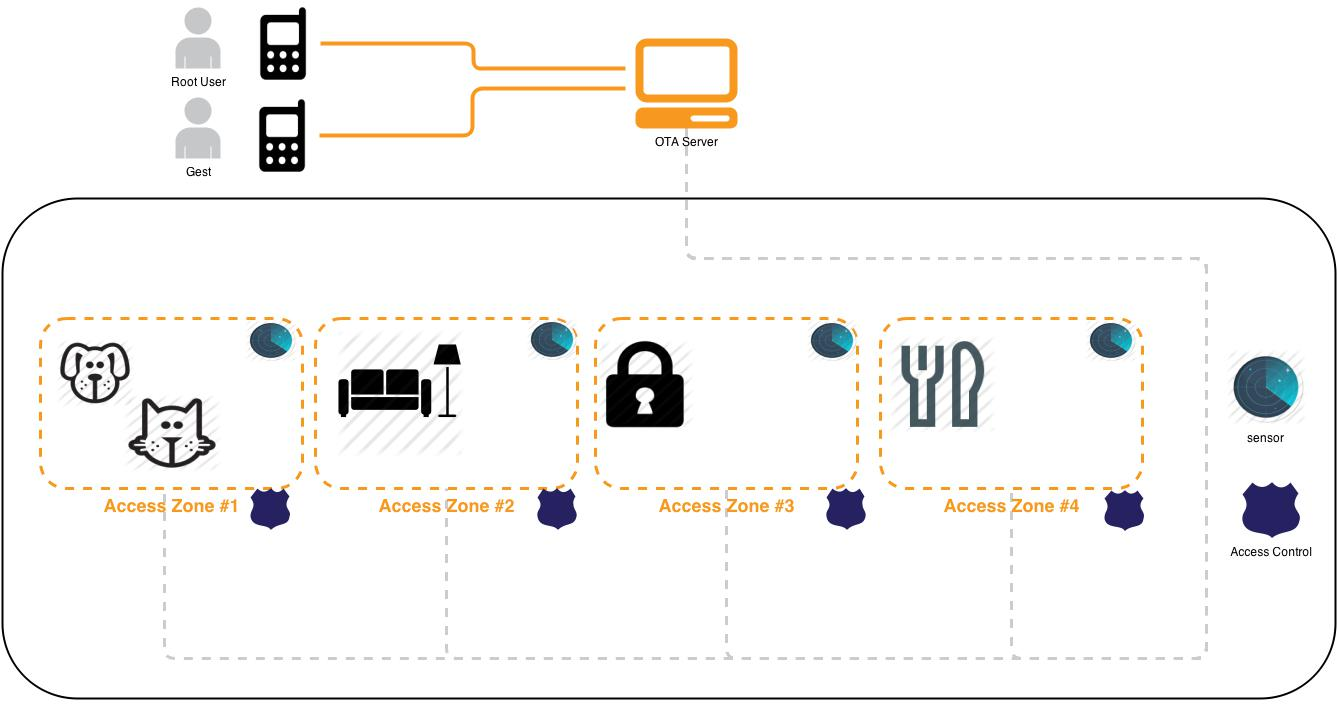
\includegraphics[width=1\textwidth]{homeoverview.jpg}
		\caption{Smart Home}
	\label{fig:SmartHome}
\end{figure}

\section{Overview}
Figure~\ref{fig:SmartHome} describes the basic structure and functionalities provided by implementation scenario Smart Home.
In the above-mentioned housing scenario, embedded with UICC smart card sensors which are in charge of monitoring and reporting environment variables, such as, home temperature, luminance and how much water the pet has, as well as embedded UICC smart card electronic device, for instance coffee maker, are deployed. On each this sensor and device an OPC UA server is installed, whose major responsibilities are controlling that corresponding device as well as managing data gathered by it.  Moreover each door in this scenario is equipped with a digital lock, that only allows user with enough authority to access. This electronic lock is also integrated with a smart card and installed the OPC UA server application. Users in this scenario can be householder or guests of home owner. Using cell phone and on this mobile terminal installed OPC UA client application, subscriber is capable of configuring sensors and querying data gathered by sensors, remote controlling aforementioned secure devices, viewing historical information recorded by corresponding facilities. With the help of such services a comfortable living condition is created in an automated way.  Moreover the root user, namely the owner of this house, is also able to assign the permission of accessing particular room to other guests. In case of when he is taking a vocation, his pet cannot get necessary care.


In this implementation scenario, OPC UA clients, namely Universal Integrated Circuit Card (UICC)  based phone user communicates with OPC UA server, which is deployed on other secure hard devices, via an OTA server.   Smart card that is applied in this scenario acts as security token for both OPC UA client and server and it contains credential information like encryption keys. certificates and digital signature. The communication stack, that manages secure  communication between OPC UA client and server application, is also developed and integrated on smart card as a Java Card applet, which means without smart card and on card Applet, OPC UA client and server are not able to appropriately finish their work.


 \begin{figure}[ht]

	\centering
	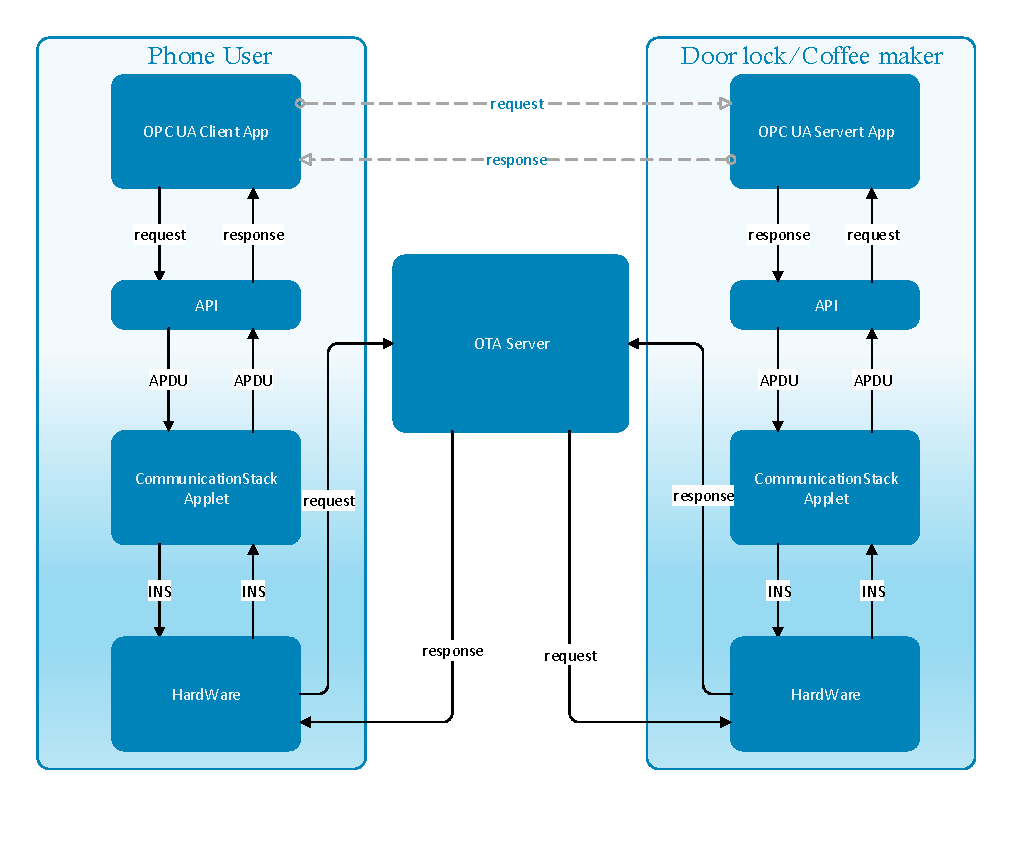
\includegraphics[width=1.1\textwidth]{csoverview}
		\caption{OPC UA Client Server Structure Example}
	\label{fig:softwareStructure}
\end{figure}


\section {Software Structure}

The whole demonstration software structure is illustrated in figure. All devices that build the system are generically referred as system components. And Components are composed of three layers. From bottom to top, they are:

\begin{itemize}
\item Physical layer. In this layer electronic devices and facilities are deployed. Alternatively lower level component could be also in this layer of higher level component.
\item Communication layer. Smart card and OPC UA client/ server application together form this layer. The main responsibility of communication layer is to create a secure communication environment for application layer.
\item Application layer. Different task and hardware specific applications reside in application layer. 
\end{itemize}

Physical layer together with communication layer create a generic platform which supports communication between different hardwares and applications. Moreover this platform also emphasizes the importance of secure messaging, peer authentication as well as authorization and provides corresponding secure mechanisms.

\subsection{Communication Flow}
Figure~\ref{fig:softwareStructure} pictures the communication flow between two system components. OPC UA Client and Server application communicate with each other with the help of an OTA server. And the communication stack is in charge of creation and managing secure communications between OTA server and secure devices. Moreover OPC UA client application is able to communicate with OPC UA server application using Short Message Service(SMS) or TCP/IP based web service. 

When the householder wants to make some coffee, he will send the \emph{makeCoffee} command to coffee maker with his cell phone. And the communication flow between two system components looks like following. Client application installed on cell phone firstly generates the \emph{makeCoffee} request and forwards it to the internal API, which translates the request into APDU and transmits this APDU command to communication stack applet. Communication stack will then creates connection with OTA server and after a successful identification OTA server will confirm the cardholder's identify and forward his request to targeted message receiver. Likewise the request message is going to be transmitted from bottom communication stack to top application step by step. At last the \emph{makeCoffee} command will be performed by coffee maker and a response message is sent back to phone user. 

\subsubsection{Conclusion}\label{secFunction}
In conclusion, server on secure device provides following services:
 \begin{itemize}
  \item processing client subscription/publishing environment data
  \item secure message exchange with client
  \item authority management
  \item historical data record
  \item execution client's command
\end{itemize}
Basic client functions as following are provided:
 \begin{itemize}
  \item submitting subscription/receiving published data
  \item secure message exchange with server
  \item sending command/configuration data
  \item querying system historical data
  \item providing user friendly interface
\end{itemize}

Communication stack is integrated in UICC smart card, whose responsibility is realizing secure channel as well as session management, transporting data to receiver using TCP/IP connections or SMS. An internal API translates OPC UA application instructions in to Application Protocol Data Unity (APDU) messages and forwards them to smart card OS, which is eventually in charge of user authentication and processing secure messaging between card application and chip card pair. 

Moreover thanks to self-containment structure, smart card itself does not dependent on other external resources, which could be extreme vulnerable to potential secure attack, and therefore provides a better hardware security and OS security. 

 \begin{figure}
	\centering
	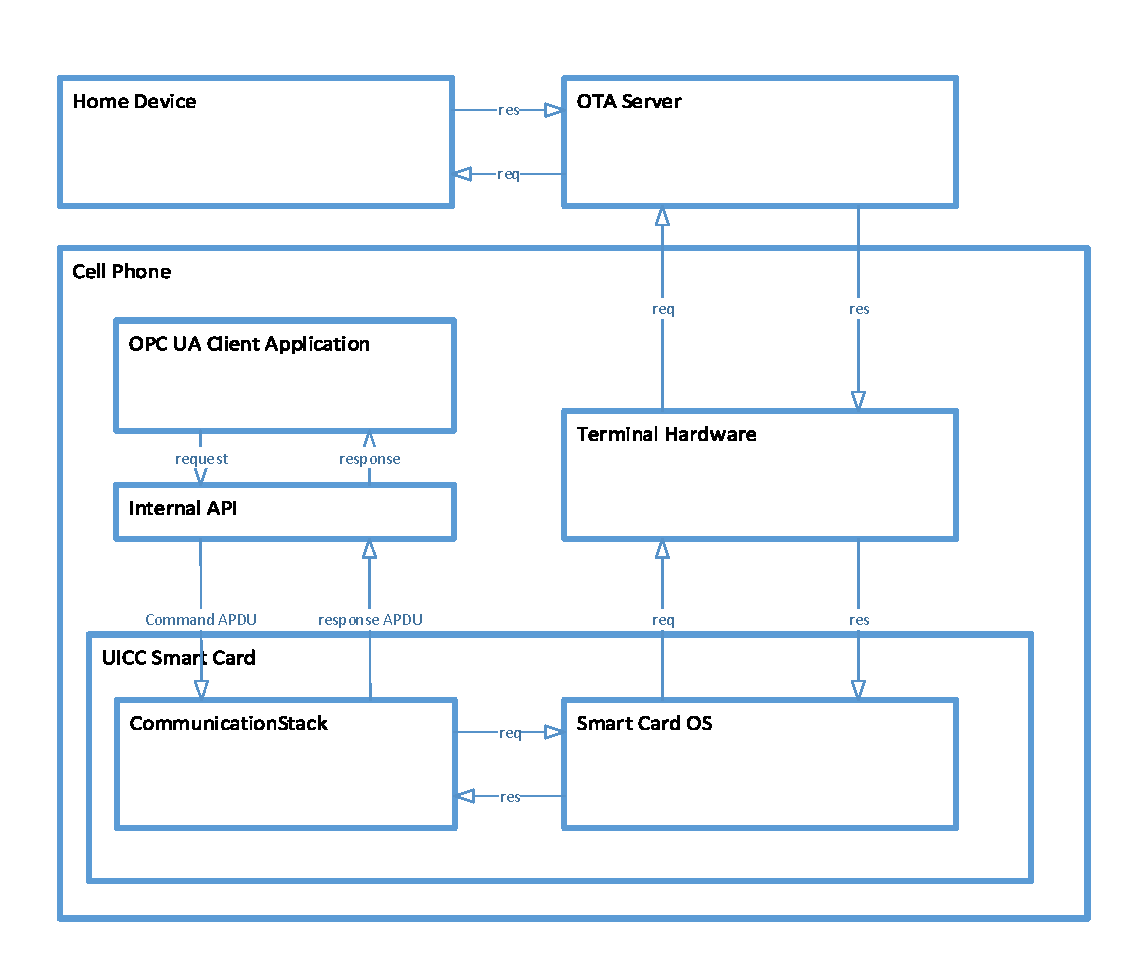
\includegraphics[width=0.78\textwidth]{clientStructure}
		\caption{Client Structure}
	\label{fig:clientStructure}
\end{figure}

\subsection{Client Structure}
As described in figure~\ref{fig:clientStructure}, the OPC UA client consists of client application code that realizes client application level functions, internal API, communication stack applet, smart card and device hardware. The Communication stack's responsibilities are:
\begin{itemize}
  \item initiate HTTP session based on TLS(proactive)
  \item trigger HTTP session based on trigger SMS send by OTA server(passive)
  \item rebuild broken communication channel
  \item message encryption as well as decryption
  \item message transmit
\end{itemize}

\begin{figure}
	\centering
	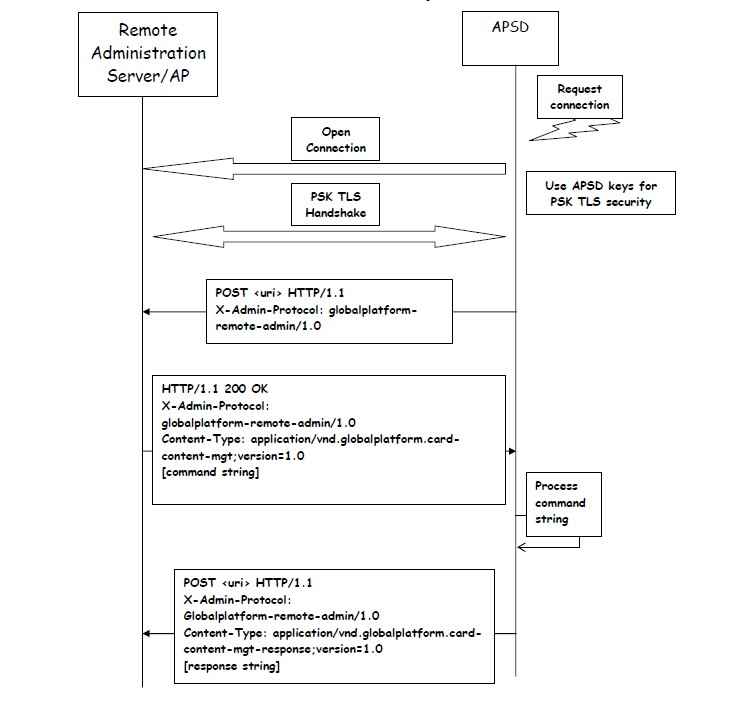
\includegraphics[width=1.2\textwidth]{apsd.jpg}
		\caption{Communication Flow between an AP and corresponding APSD\cite{ramGP}}
	\label{fig:apsd}
\end{figure}
The communication flow compliant with the one provided by GlobalPlatform, which provides mechanisms that allow secure information exchanged between a remote entity and a terminal, this process is also known as Remote Application Management(RAM) over HTTP protocol and PSK TLS security. The on card component, which is responsible for connection creation with the remote entity and user/application authentication, is called Security Domain(SD). And the aforementioned remote entity  is  referred as Remote Administration Server as well. With these concepts, smart card with Security Domain issued  by GloablPlatform can act as HTTP client and is capable of packing APDU formate information into HTTP POST message and transmitting HTTP message to OTA server, which will then forward this HTTP message to target receiver.\cite{ramGP}
 
Figure~\ref{fig:apsd} illustrates a typical communication flow between administration server and corresponding security domain (Application Security Domain) on smart card. As can be seen, the request for open communication is usually initialized by security domain, which is also the phone user. After a successful creation of secure handshake, the remote administration server and security domain are able to based on HTTP connection exchange request and response strings, which encapsulate APDU instructions. GlobalPlatform has also provided  a lists of API used to initialize authentication process, to configure algorithm and keys for message encryption and decryption, to perform secure messaging and etc.

\subsection{Server Structure}

\begin{figure}
	\centering
	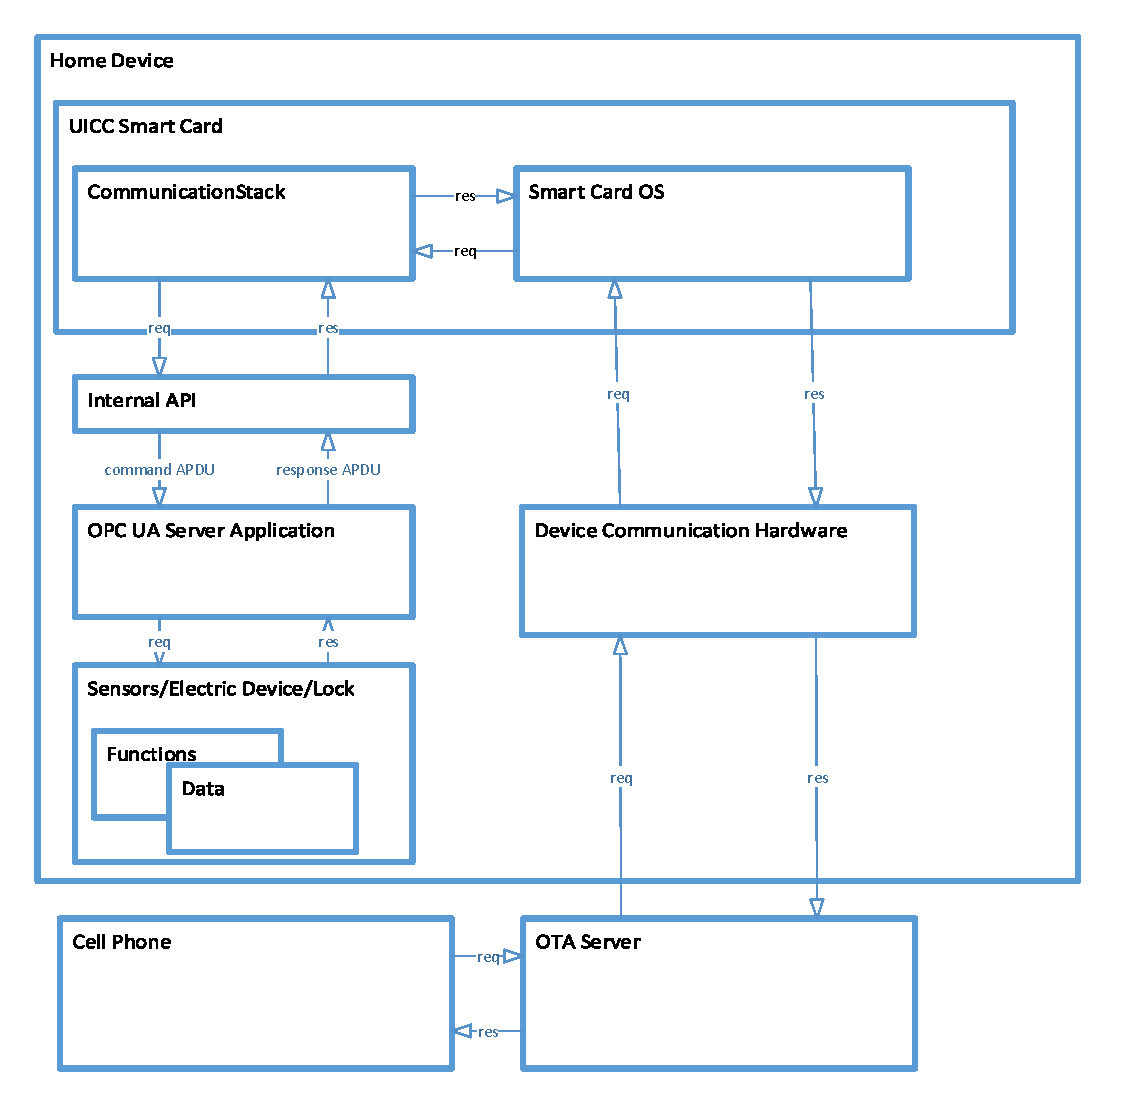
\includegraphics[width=0.95\textwidth]{serverStructure}
		\caption{Server Structure}
	\label{fig:serverStructure}
\end{figure}
Server here refers sensors, electric device as well digital locks that together build up the smart home system. Each server controls exactly one above-mentioned secure device and take subscription as well as publish corresponding notification to authenticated subscriber. The server structure is pictured as figure~\ref{fig:serverStructure} and it consists of OPC UA server application code, which offers basic services like subscription and notification mentioned before, an internal API, an on smart card integrated communication stack and functions as well as data provided by corresponding facility.

\subsection{Implementation Tool Support}
\subsubsection{Java Card Application Design and Debug Tool}
Morpho presents JACADE with full name, Java Card Applet Develop Environment, which is more than just a IDE but a complex selection of various class APIs and software modules, that can be applied to design complete Java Card Applet as well as to debug Java source. 
\subsubsection{Java Card Applet Testing Environment}
When it comes to running test with Java Card Applet, tester has two options. Firstly, he can install the to be tested Applet on a smart card and then connection this chip card with test computer using \emph{Morpho Card Reader (MCR)}. Alternatively \emph{Java virtual card} which is integrated test Applet also could be applied. 

In either way, as next step \emph{Universal Test Environment (UTE)} will be applied. \emph{UTE} provided by Morpho uses Java languages developed test cases
 and test scenarios\footnote{Test scenario is a collection of relative test cases.} to simulate desired use cases and observe corresponding smart card reactions. With the observed test result, tester will be able to analyze Applet's performance and debug corresponding application code. For instance \emph{UTE} can integrate software models used to simulate security domain offered by \emph{Globalplatform} and perform the sophisticate user authentication simulation process.
\subsubsection{Android Application Design Tool}
Eclipse IDE for Java Developer of version 3.7.1 is applied ,together with Android SDK \emph{seek-for-android} and ADT plug-in, as Android Application development environment. Android 2.3.5 is simulated and chosen as demonstration platform.
\subsubsection{Smart Home Simulation Environment}
In order to simulate data manged by home electronic device, \emph{MySQL} database is introduced. And together with \emph{PHP of version 5.5.12}, \emph{Apache of version 2.4.9}, the web server for Smart Home is created. Android Application from previous subsection will then communication with this web server for the purpose of scenario demonstration.
\clearemptydoublepage
\chapter{System Design}

\begin{figure}[!htbp]
	\centering
	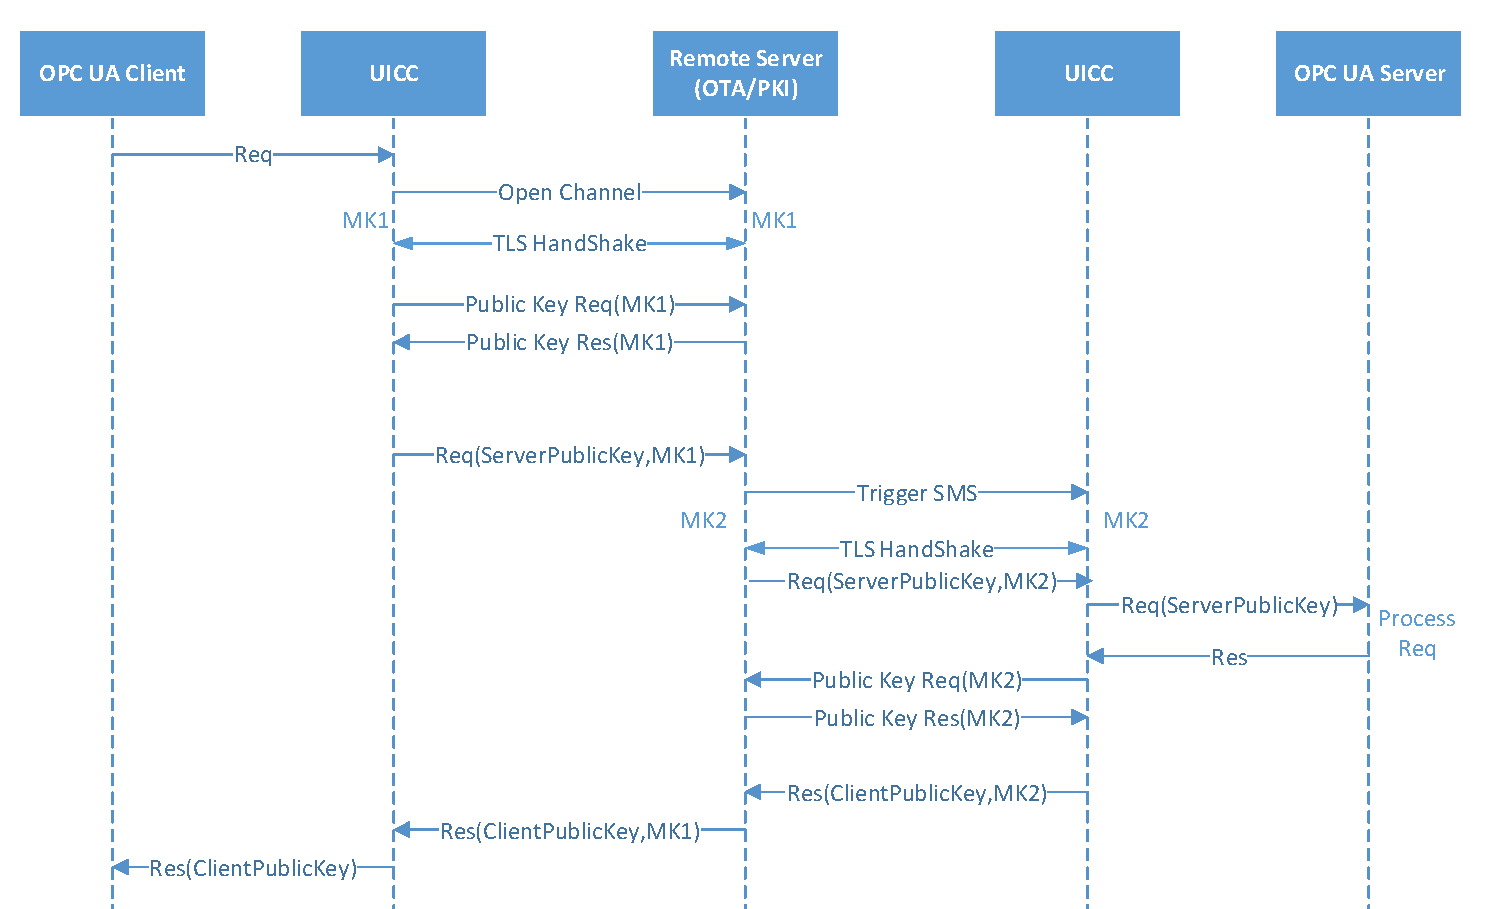
\includegraphics[width=1\textwidth]{whole-structure}
		\caption{Message Exchange}
	\label{fig:whole-structure}
\end{figure}

As described in previous sections, my demonstration system consists of three main parts, namely the on card integrated communication stack, Android application and Smart Home web service. Figure~\ref{fig:whole-structure} illustrates the request and corresponding response message exchange process that occurs in the demonstration system. In my case I integrate \emph{Public Key Infrastructure} with OTA server, in order to perform secure peer identification and messaging.
\section{Overview}
The whole message exchange process consists of following phases:
\begin{itemize}
\item \emph{Open Channel Phase} Whenever a OPC UA client/server attempts to contact with other housing devices or Remote Server tries to communicate with a home device, a communication session between Remote Server and home device must be created.
\item \emph{TSL Handshake with Remote Server} After a successful creation of communication channel, a mutual peer identification through TLS handshake between Remote server and aforementioned client/server will be performed.
\item \emph{Require target's public key} When Remote Server identify the connected communication partner, it will grant client/server the expected target's public key. 
\item \emph{secure messaging} Message sender will in this phase encrypt message with target's public key and send this encrypted message through Remote Server to message receiver. 
\end{itemize}

\section{UICC Applet}

\subsection{Classes}\sloppy
My UICC applet is integrated in Morpho \emph{SC5-01OS07} LTE SAT product.
Communication stack includes following classes:
 \begin{itemize}
  \item  \emph{CommunicationStack}, which is the main class of my applet, that implements \emph{install}, \emph{select}, \emph{deselect} as well as \emph{process} methods provided by \emph{javacard.framework.Applet}. In order to process remote APDU, this applet is also design as UICC system applet, that extends interface \emph{com.orga.javacard.componentinterfaces.JCISIMApplication}
  \item  \emph{AdminTrigger}, which implements Globalplatform  and toolkitframework interfaces and offers functions for proactive and passive communication session creation with OTA server, cipher suit negotiation and mutual authentication.
\end{itemize}

\begin{figure}[!htbp]
	\centering
	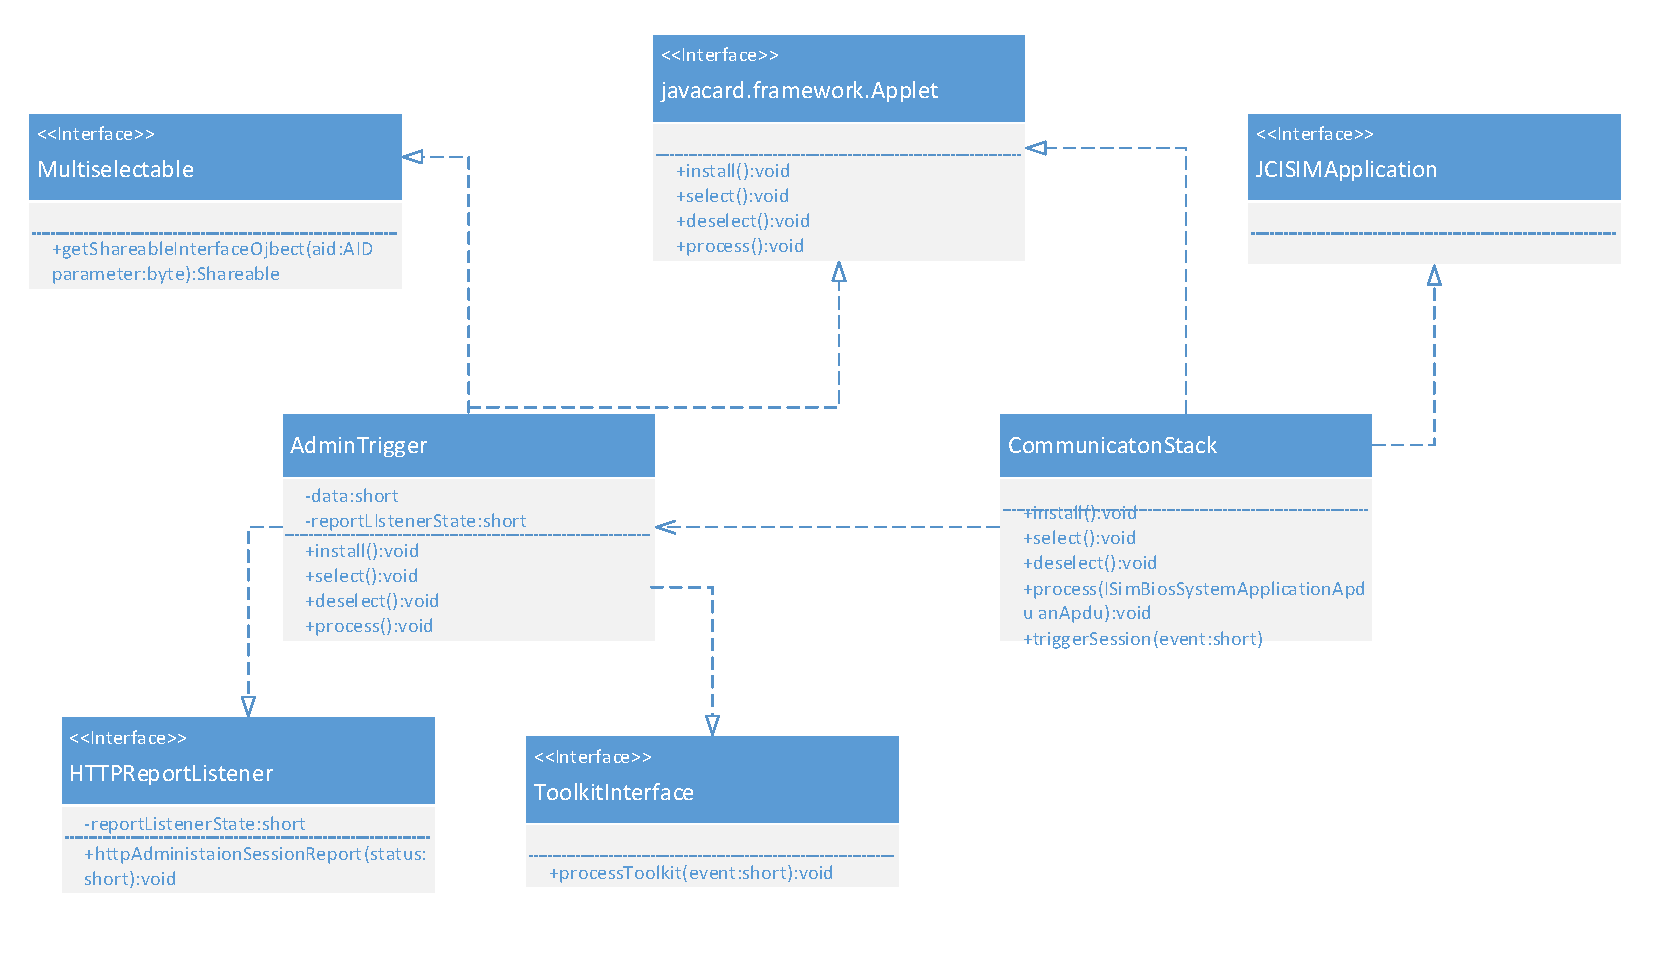
\includegraphics[width=1.0\textwidth]{class}
		\caption{Class Diagram}
	\label{fig:class}
\end{figure}

\subsection {Work Flow}

The components involved in this scenario are:
 \begin{itemize}
  \item CommunicationStack applet and associated Security Domain from Globalplatform (APSD  for short)
  \item OTA server which is also known as Remote Administration Server (RAS for short)
\end{itemize}

The communication between CommunicationStack and Remote Administration Server involves following  steps:

 \begin{itemize}
  \item Open Communication Channel and Create Communication Session
  \item Secure Message Exchange
  \item Close Communication Session
\end{itemize}
\subsubsection{Communication Session Creation and Message Exchange}
This process could be either initiated by Remote Administration Server by sending target applet a trigger SMS or be sponsored by applet itself. In both cases, applet sends the first \emph{OpenChannel Request} message. During the PSK TLS Handshake phase, APSD and remote server will agree on to be used cipher suit and authenticate each other. After a successful PSK TLS Handshake, CommunicationStack and remote OTA server will be able to exchange HTTP message, which encapsulates APDU strings as body. And HTTP header is in compliance with GlobalPlatform standards.


\begin{figure}[!htbp]

	\centering
	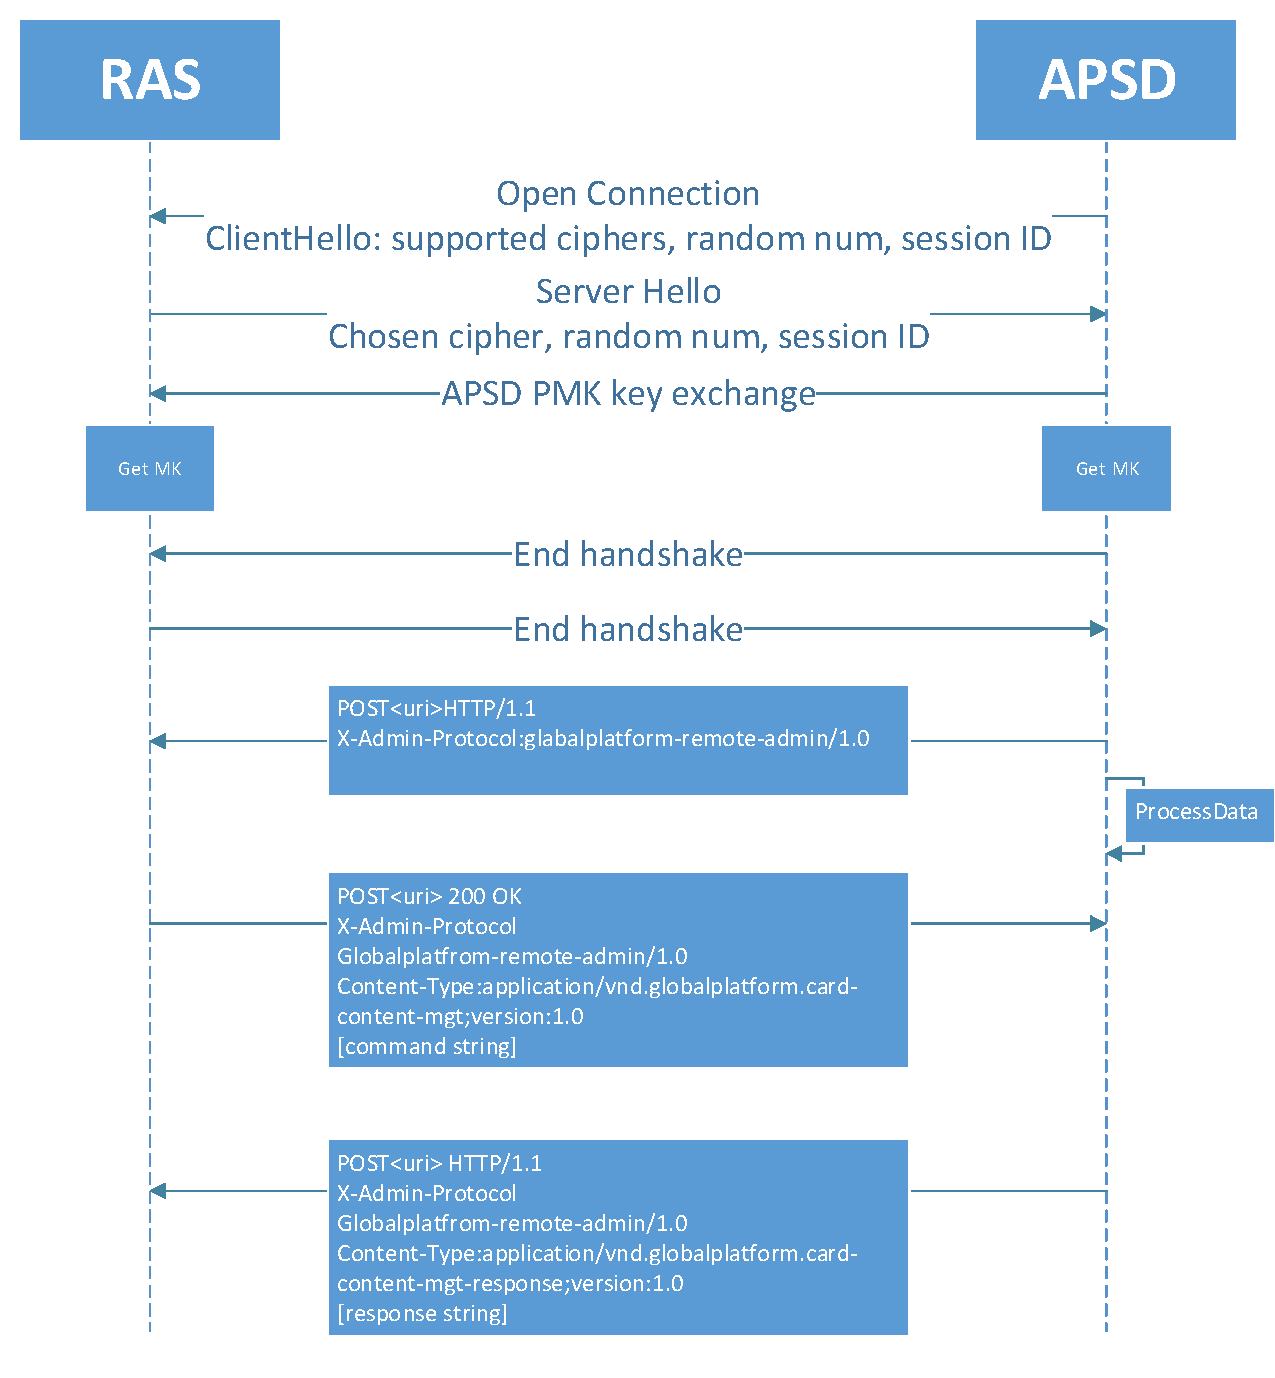
\includegraphics[width=1\textwidth]{communication-flow}
		\caption{Handshake and message exchange between SD and Remote Server}
	\label{fig:communication-flow}
\end{figure}

\subsubsection{HTTP Header Format}
The HTTP message sent from remote sever to targeted applet uses following schema\cite{gp}:
\begin{verbatim}
HTTP/1.1 200 OK [or HTTP/1.1 204 No Content CRLF]
X-Admin-Protocol: globalplatform-remote-admin/1.0 CRLF
[X-Admin-Next-URI:  <next-URI> CRLF]
[Content-Type: application/vnd.globalplatform.card-content-mgt
-response;version=1.0 CRLF]
[X-Admin-Targeted-Application: <security-domain-AID> CRLF]
[Content-Length: xxxx CRLF] or [Transfer-Encoding: chunked CRLF]
CRLF
[body]
\end{verbatim}
The field \emph{security-domain-AID} will be filled with the AID of targeted applet.


The HTTP response message sent from applet to remote server uses following schema\cite{gp}:
\begin{verbatim}
POST<URI>HTTP/1.1 CRLF
Host: <Administration Host> CRLF
X-Admin-Protocol: globalplatform-remote-admin/1.0 CRLF
X-Admin-From: <Agent ID> CRLF
[Content-Type: application/vnd.globalplatform.card-content-mgt
-response;version=1.0 CRLF]
[Content-Length: xxxx CRLF] or [Transfer-Encoding: chunked CRLF]
[X-Admin-Script-Status: <script-status> CRLF]
[X-Admin-Resume: true]
CRLF
[body]
\end{verbatim}

The filed \emph{X-Admin-Script-Status} could contain following values:
 \begin{itemize}
  \item \emph{ok}, which means that the previous message is successfully received by applet.
  \item \emph{unknown-application}, which stands for the error, that the targeted applet for previous message can not be found.
\item \emph{not-a-security-domain}, this errors occurs when targeted applet is not a Security Domain.
\item \emph{security-error}, as its name indicates, this values is returned if the security of previous message  can not be checked.
\end{itemize}

\subsubsection{Close Communication Session}
Whenever the communication channel is about to be closed, either because of session security issue, or due to successful finish of communication, remote server will send target applet HTTP message using following parameters:
 \begin{itemize}
  \item No \emph{X-Admin-Next-URI} field is present in this HTTP message and message body is empty, which will be recognized as final message from remote server and then the session will be closed.
  \item No \emph{X-Admin-Next-URI} filed is present but in this HTTP message body is not empty. The receiver will process the data in body and close the communication session appropriately. But no response message will be generated.
\end{itemize}

\subsection {Commands: Interface between Applet and CAD}
Before concrete implementation of Javacard applet code, the interface, which in essence is a set of commond APDUs and corresponding response APDUs, between applet and CAD must be well defined.  The CommunicationStack support two categories commond APDU:
 \begin{itemize}
  \item The \emph{SELECT} Command APDU, which is used by JCRE to select CommunicationStack applet.
  \item Other command APDUs, which are introduced in order to provide functionalists such as: trigger communication session, process input APDU and etc. To be more specifically:
\begin{itemize}
  \item PIN operation related APDU set
  \item Communication session management APDU set
  \item Data process APDU set
\end{itemize}
\end{itemize}

\subsubsection{SELECT APDU}
The header of this command APDU is fixed and \emph{Lc} indicates the length of CommunicationStack AID. In \emph{Data filed} real AID is saved.
\begin{table}[!htbp]
\caption{SELECT command APDU}
\scalebox{0.8}{%
\begin{tabular}{|l|l|l|l|l|l|l|}
\hline
CLA  & INS  & P1   & P2   & Lc   & Data field                                                                                          & Le  \\ \hline
0x00 & 0xA4 & 0x04 & 0x00 & Length of AID& AID & N/A \\ \hline
\end{tabular}
}
\label{select-apdu}
\end{table}
Two categories of response APDUs are expected, one represents successful processing of \emph{SELECT} command APDU and the other stands for failure.
\begin{table}[!htbp]
\caption{SELECT response APDU}
\label{select-response-apdu}
\scalebox{0.8}{%
\begin{tabular}{|l|l|l|}
\hline
Optional data & Status word & Description                                \\ \hline
No data       & 0x9000      & Successful processing                      \\ \hline
              & 0x6999      & Failed to select CommunicationStack applet \\ \hline               
\end{tabular}
}
\end{table}

\subsubsection{Verify PIN operation}
This APDU command and response set is used to let CommunicationStack applet verify identity of terminal user. Moreover the PIN size is set from four to eight and the verify PIN operation only allows three times wrong PIN input before a successful identification.

\begin{table}[!htbp]
\caption{Verify PIN command }
\scalebox{0.8}{%
\begin{tabular}{|l|l|l|l|l|l|l|}
\hline
CLA  & INS  & P1   & P2   & Lc   & Data field    & Le  \\ \hline
0xA0 & 0x11 & 0x00 & 0x00 & length of Data field & PIN & N/A \\ \hline
\end{tabular}
}
\label{verify-command-apdu}
\end{table}

As described in tabl~\ref{verify-response-apdu}, three categories of response APDUs are expected.

\begin{table}[!htbp]
\caption{Verify PIN response APDU}
\label{verify-response-apdu}
\scalebox{0.8}{%
\begin{tabular}{|l|l|l|}
\hline
Optional data & Status word & Description                                \\ \hline
No data       & 0x9000      & Successful processing                      \\ \hline
              & 0x63C0      & Verification failed \\ \hline      
              & 0x6983      & After 3 times wrong input, PIN is block \\ \hline              
\end{tabular}
}
\end{table}

\subsubsection{Reset PIN operation}
This APDU command and response set is introduced to offer end user change PIN service.

\begin{table}[!htbp]
\caption{Reset PIN command }
\scalebox{0.8}{%
\begin{tabular}{|l|l|l|l|l|l|l|}
\hline
CLA  & INS  & P1   & P2   & Lc   & Data field    & Le  \\ \hline
0xA0 & 0x12 & 0x00 & 0x00 & length of Data field &New PIN & N/A \\ \hline
\end{tabular}
}
\label{reset-pin-command-apdu}
\end{table}

Three categories of response APDUs are expected.
\begin{table}[!htbp]
\caption{Reset PIN response APDU}
\label{reset-pin-response-apdu}
\scalebox{0.8}{%
\begin{tabular}{|l|l|l|}
\hline
Optional data & Status word & Description                                \\ \hline
No data       & 0x9000      & Successful processing                      \\ \hline
              & 0x6301      & Verification is required first\\ \hline      
              & 0x6984      & Length of input PIN is wrong \\ \hline              
\end{tabular}
}
\end{table}


\subsubsection{Communication Session Creation}
\begin{table}[!htbp]
\caption{Communication session creation command APDUs}
\scalebox{0.75}{%
\begin{tabular}{|l|l|l|l|l|l|l|l|}
\hline
CLA  & INS  & P1   & P2   & Lc   & Data field  & Le  & Description \\ \hline
0xA0 & 0x01 & 0x00 & 0x00 & data filed length & Session parameter& N/A  & create session parameters\\ \hline
0xA0 & 0x02 & 0x00 & 0x00 & data filed length & Session parameter& N/A  & set session parameters\\ \hline
0xA0 & 0x03 & 0x00 & 0x00 &  N/A & N/A& N/A  & create communication session\\ \hline
0xA0 & 0x04 & 0x00 & 0x00 &  N/A & N/A& length of session state & get session state\\ \hline
\end{tabular}
}
\label{trigger-session-apdu}
\end{table}
This APDU command and response set is used to let  CommunicationStack applet initiate the request to establish communication channel and create communication  session above  it. Following commands are supported.



Following return codes are expected in response APDU:

.\begin{table}[!htbp]
\caption{Trigger Session Return Code}
\label{trigger-session-response-apdu}
\scalebox{0.8}{%
\begin{tabular}{|l|l|l|}
\hline
 Status word & Description                                \\ \hline
 0x9000      & Successful processing                      \\ \hline
 0x66AB      & Array Index out of bounds exception \\ \hline           
 0x665E      & Security exception \\ \hline 
 0x6600      & Nullpointer  exception \\ \hline  
 0x6C00      & UnKnown  exception \\ \hline      
\end{tabular}
}
\end{table}


\subsubsection{Close Communication Session }
This APDU command and response set is used to correctly close  communication channel.


\begin{table}[!htbp]
\caption{Close Session command APDU}
\scalebox{0.8}{%
\begin{tabular}{|l|l|l|l|l|l|l|}
\hline
CLA  & INS  & P1   & P2   & Lc   & Data field                                                                                          & Le  \\ \hline
0xA0 & 0x50 & 0x00 & 0x00 & 0x00 & N/A& N/A \\ \hline
\end{tabular}
}
\label{close-session-apdu}
\end{table}

Following return codes are expected in response APDU:

.\begin{table}[!htbp]
\caption{Close Session Return Code}
\label{close-session-response-apdu}
\scalebox{0.8}{%
\begin{tabular}{|l|l|l|}
\hline
 Status word & Description                                \\ \hline
 0x9000      & Successful processing                      \\ \hline
 0x6032      & Failed to close session \\ \hline             
\end{tabular}
}
\end{table}

\subsubsection{Process Communication Data }
\begin{table}[!htbp]
\caption{Process data command APDUs}
\scalebox{0.8}{%
\begin{tabular}{|l|l|l|l|l|l|l|l|}
\hline
CLA  & INS  & P1   & P2   & Lc   & Data field  & Le \\ \hline
0xA0 & 0x20 & 0x00 & 0x00 & data filed length & desired target's public key & PK length \\ \hline
0xA0 & 0x21 & 0x00 & 0x00 & data filed length & command data & response length \\ \hline
\end{tabular}
}
\label{process-data-cmd-apdu}
\end{table}
This APDU command and response set is used to provide functionalities to perform command processing between cellphone and  other smart home device. 

.\begin{table}[!htbp]
\caption{Process data Return Code}
\label{process-data-res-apdu}
\scalebox{0.8}{%
\begin{tabular}{|l|l|l|}
\hline
 Status word & Description                                \\ \hline
 0x9000      & Successful processing                      \\ \hline
 0x6A80      & error in data filed \\ \hline        
 0x6A81      & required device not found \\ \hline        
 0x6A82      & required service not found \\ \hline   
 0x6A83      & required record not found \\ \hline                
\end{tabular}
}
\end{table}
Following return codes as shown in table~\ref{process-data-res-apdu} are expected in response APDU.

Moreover \emph{command data} in data filed of command APDU adopts following TLV format. 

\section{Android Application}
\section{Smart Home Web Server}
\clearemptydoublepage
\chapter{Implementation Test}
In this chapter, a brief demonstration testing cases are presented. To be more specifically, two testing scenarios related with \emph{CommunicationStack} applet and simulated remote server are designed. At the same time, the testing cases demonstrating communication between Smart Home web server component and Android application are designed.

\section{Remote Management Testing}
The aim of this testing scenario is to prove the feasibility of applying Smart Card and remote application/file management protocols proposed by Globalplatform to provide a secure dual authentication and messaging platform for other 
higher leveled applications. My Javacard Applet, \emph{CommunicationStack} together with correspondingly designed \emph{UTE} test cases are employed and build the testing environment.

\subsection{\emph{UTE} Test Case}

Two \emph{UTE} test cases are programmed. They are:
\begin{itemize}
\item \emph{Trigger Communication Channel with SMS}. In this test case, I simulate the open communication channel process between smart card and remote administrator server. This process is also the cornerstone for a successful remote application management.
\item \emph{Secure Messaging Exchanging} After a successful identification between communication peers and creation of communication channel, in this test scenario, smart card and remote server are going to perform secure messaging. 
\end{itemize}

\subsubsection{Trigger Communication Channel with SMS} \label{secAppletTest1}
In this test suit, UTE testing case acts as a remote administrator server and encapsulates information necessary for the construction of a secure Http channel in a \emph{TriggerPushSMS} object and sent this SMS to target smart card applet using simulated GPRS connection. The SMS structure is pictured in figure~\ref{fig:push-sms} and includes parameters which are categorized as following:
\begin{figure}[!htb]
	\centering
	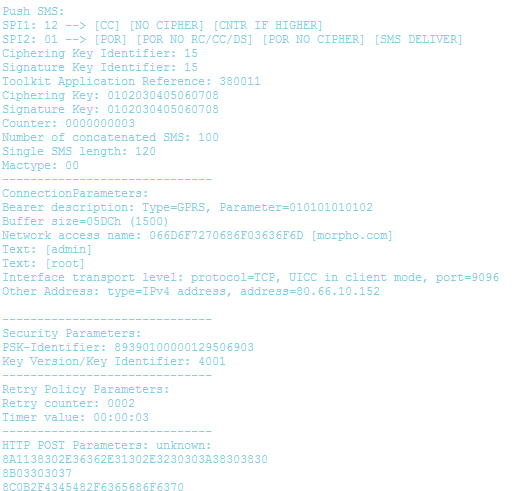
\includegraphics[width=1.0\textwidth]{Images/impl/push-sms.png}
		\caption{Push Short Message including all parameters which are necessary for the creation of communication channel}
	\label{fig:push-sms}
\end{figure}
\begin{itemize}
\item \emph{Connection Parameters}, which includes network access name, bearer description and other parameters describing the simulated remote server.
\item \emph{Security Parameters} In security parameters, proposed TLS 1.2 connection information, such as suggested cipher suit, is provided
\item \emph{Smart Card Keysets}, that consists of key identifiers as well as indicator used for the select of cipher keys and signature keys.
\item \emph{Http connection parameters}. Also parameters such as retry counter, timeout values are included in this short message.
\end{itemize}
After a successful receiving and processing of aforementioned push SMS, \emph{CommunicationStack} will preform TLS handshake with the remote server. 

The TLS \emph{client hello} is demonstrated by figure~\ref{fig:client-hello}. And in this demonstration case \emph{TLS\_PSK\_WITH\_NULL\_SHA256} is chosen. At last, the master key, shown in figure~\ref{fig:mk} is generated between remote server and card applet.

\begin{figure}[!htb]
	\centering
	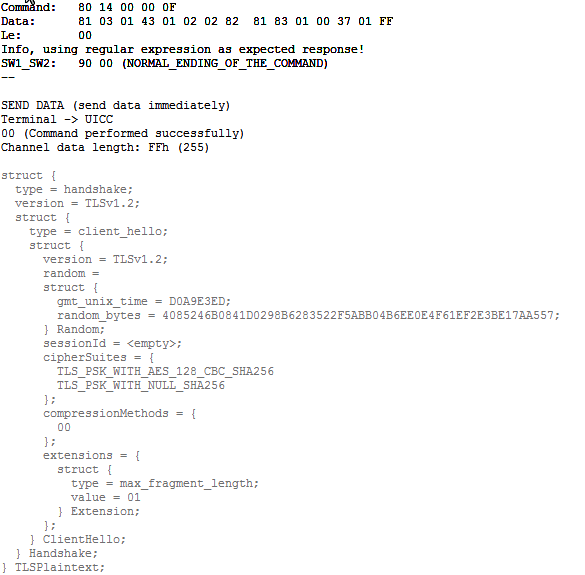
\includegraphics[width=1\textwidth]{Images/impl/client-hallo.png}
		\caption{TLS client hello sent by smart card applet}
	\label{fig:client-hello}
\end{figure}

\begin{figure}[!htb]
	\centering
	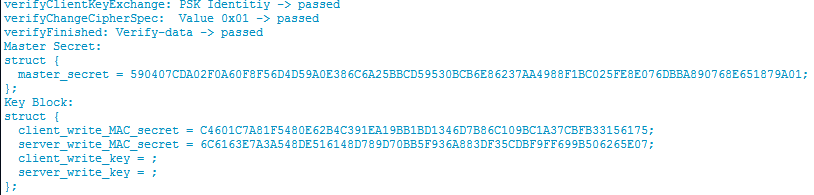
\includegraphics[width=1\textwidth]{Images/impl/master-key.png}
		\caption{Successful generation of master key between remote server and \emph{CommunicationStack} applet}
	\label{fig:mk}
\end{figure}


\subsubsection{Secure Messaging Exchanging}

\begin{figure}[!htb]
	\centering
	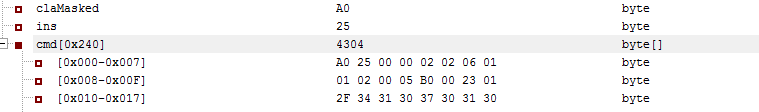
\includegraphics[width=1.2\textwidth]{Images/impl/cmd.png}
		\caption{\emph{cmd} Buffer in \emph{CommunicationStack} applet.}
	\label{fig:remote1}
\end{figure}

Based on in previous paragraph ~\ref{secAppletTest1} created secure channel and Http Connection, in this test case, smart card applet and remote server perform secure message exchange. As illustrated in figure~\ref{fig:remote1}, my applet is able to receive Http Message from remote server and retrieve the encapsulated command data. Furthermore as shown in figure~\ref{fig:remote2}, at the end of this testing scenario, remote server receives a Http message from \emph{CommunicationStack} and the content of this message is apparently secured, whose clear test is presented in figure~\ref{fig:remote2}.

\begin{figure}[!htb]
	\centering
	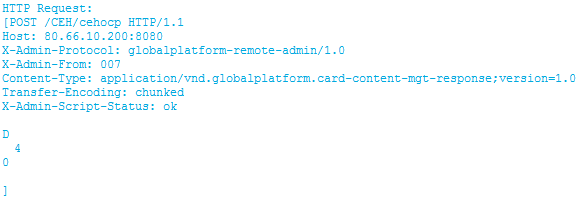
\includegraphics[width=1\textwidth]{Images/impl/http-msg.png}
		\caption{Http Response Message received by remote server}
	\label{fig:remote2}
\end{figure}

\begin{figure}[!htb]
	\centering
	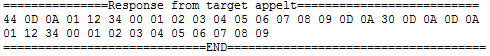
\includegraphics[width=0.85\textwidth]{Images/impl/translate.png}
		\caption{Http Content Translation}
	\label{fig:remote3}
\end{figure}

\begin{figure}[!htb]
\begin{minipage}{0.49\linewidth}
  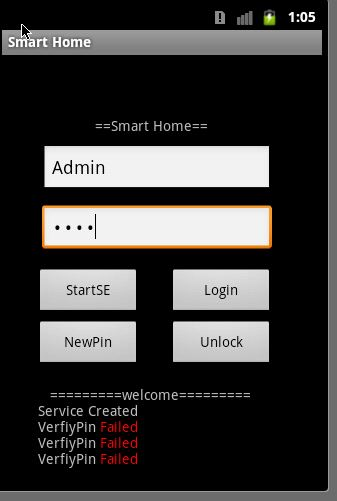
\includegraphics[width=0.8\linewidth]{Images/impl/3failed.jpg}
  \caption{Wrong PIN input}
  \label{fig:sub1}
\end{minipage}
    \hfill
\begin{minipage}{0.49\linewidth}
  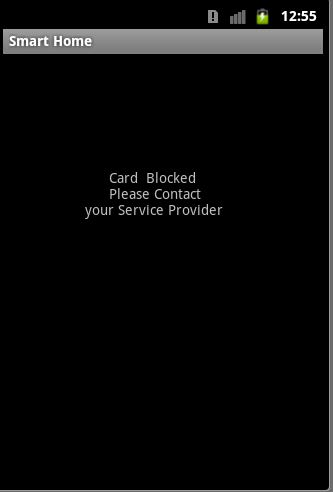
\includegraphics[width=0.8\linewidth]{Images/impl/UI3.jpg}
  \caption{PIN is blocked}
  \label{fig:sub2}
\end{minipage}
  \end{figure}
\section{Android Application Testing}
In this section, how my Android application interact with Smart Home web server and smart card applet will be demonstrated.

\subsection{PIN Verification}

As already introduced, in order to use functionalities provided by Smart Home, phone holder must authenticate himself by inputing PIN for Android application. But after three times wrong PIN input, as shown in figure~\ref{fig:sub1}, PIN will be locked. And only the service provider can unblock this PIN. 
\subsection{Communication with Web server}
After a successful identification, Android application user now can enjoy functions provided by Smart Home application, such as remote housing device management and querying historical data, as shown in following figures.

\begin{figure}[!htb]
	\centering
	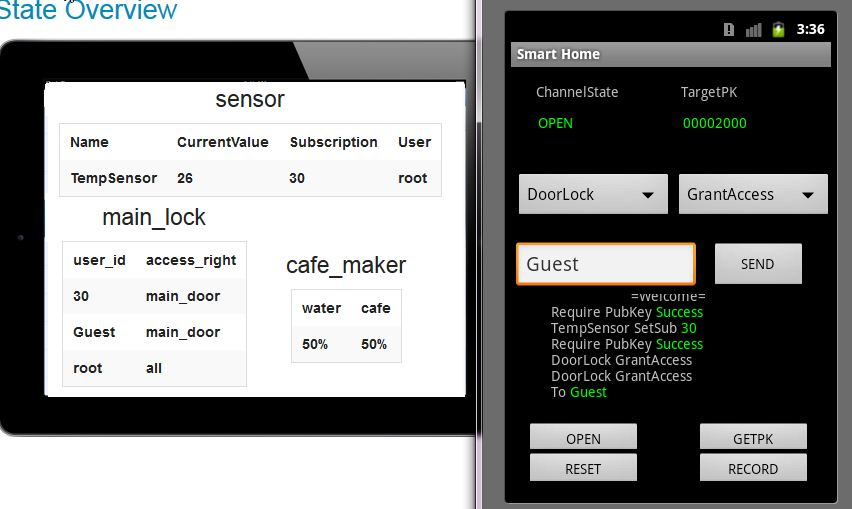
\includegraphics[width=0.85\textwidth]{Images/impl/housing-device.jpg}
		\caption{Using Android application remotely managing home devices}
	\label{fig:housing-device}
\end{figure}

\begin{figure}[!htb]
	\centering
	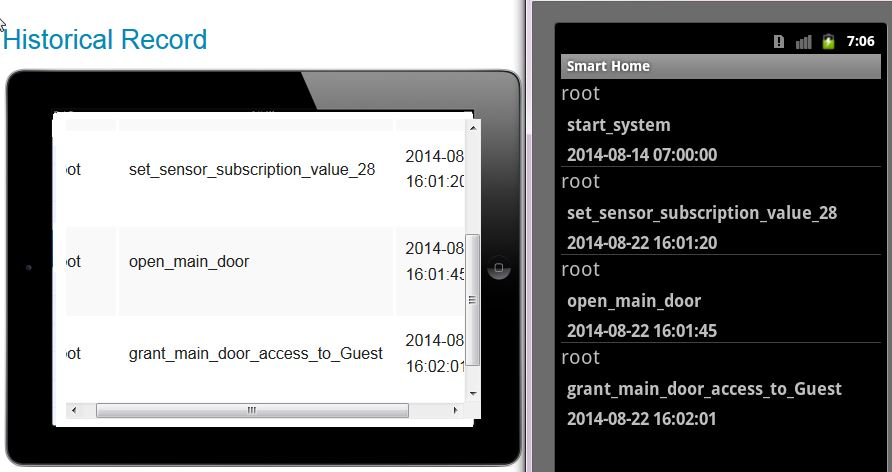
\includegraphics[width=0.85\textwidth]{Images/impl/record-query.jpg}
		\caption{Historical Record Overview}
	\label{fig:record-query}
\end{figure}

\clearemptydoublepage
\chapter{System Security Analysis}
In this chapter, I will perform a secure analysis based on the demonstration system described early for the purpose of confirming the feasibility of my proposal. To be more specifically, I am going to introduce a conceptional attack tree graph, with whose help the potential threats and attacks aiming at my system are analyzed. Moreover for each type of threads, i will proof that there exits at least one secure countermeasure in my system.

\section{Attack Tree Overview}

 \begin{figure}[!htb]
	\centering
	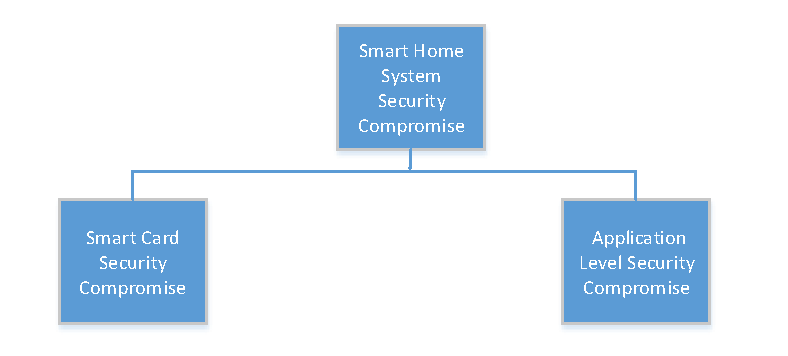
\includegraphics[width=0.85\textwidth]{attack-tree-overview}
		\caption{Attack tree overview}
	\label{fig:attack-tree-overview}
\end{figure}
As shown in figure~\ref{fig:attack-tree-overview} the attack tree is categorized into two main sub attack  trees. The first type group describes attacks that the third malicious party could apply to harm the smart card employed in my scenario. And the second ones contain higher application level related threats, namely the security threats to OPC UA standards and applications. 

\section{Smart Card Security Compromise}
In this section, I will firstly present the attack tree in the domain of smart card and based on this attack tree  perform the secure analysis . At last countermeasures designed and integrated in my system is going to be described.

\subsection{Sub Attack Tree and its Content}
 \begin{figure}[!htb]
	\centering
	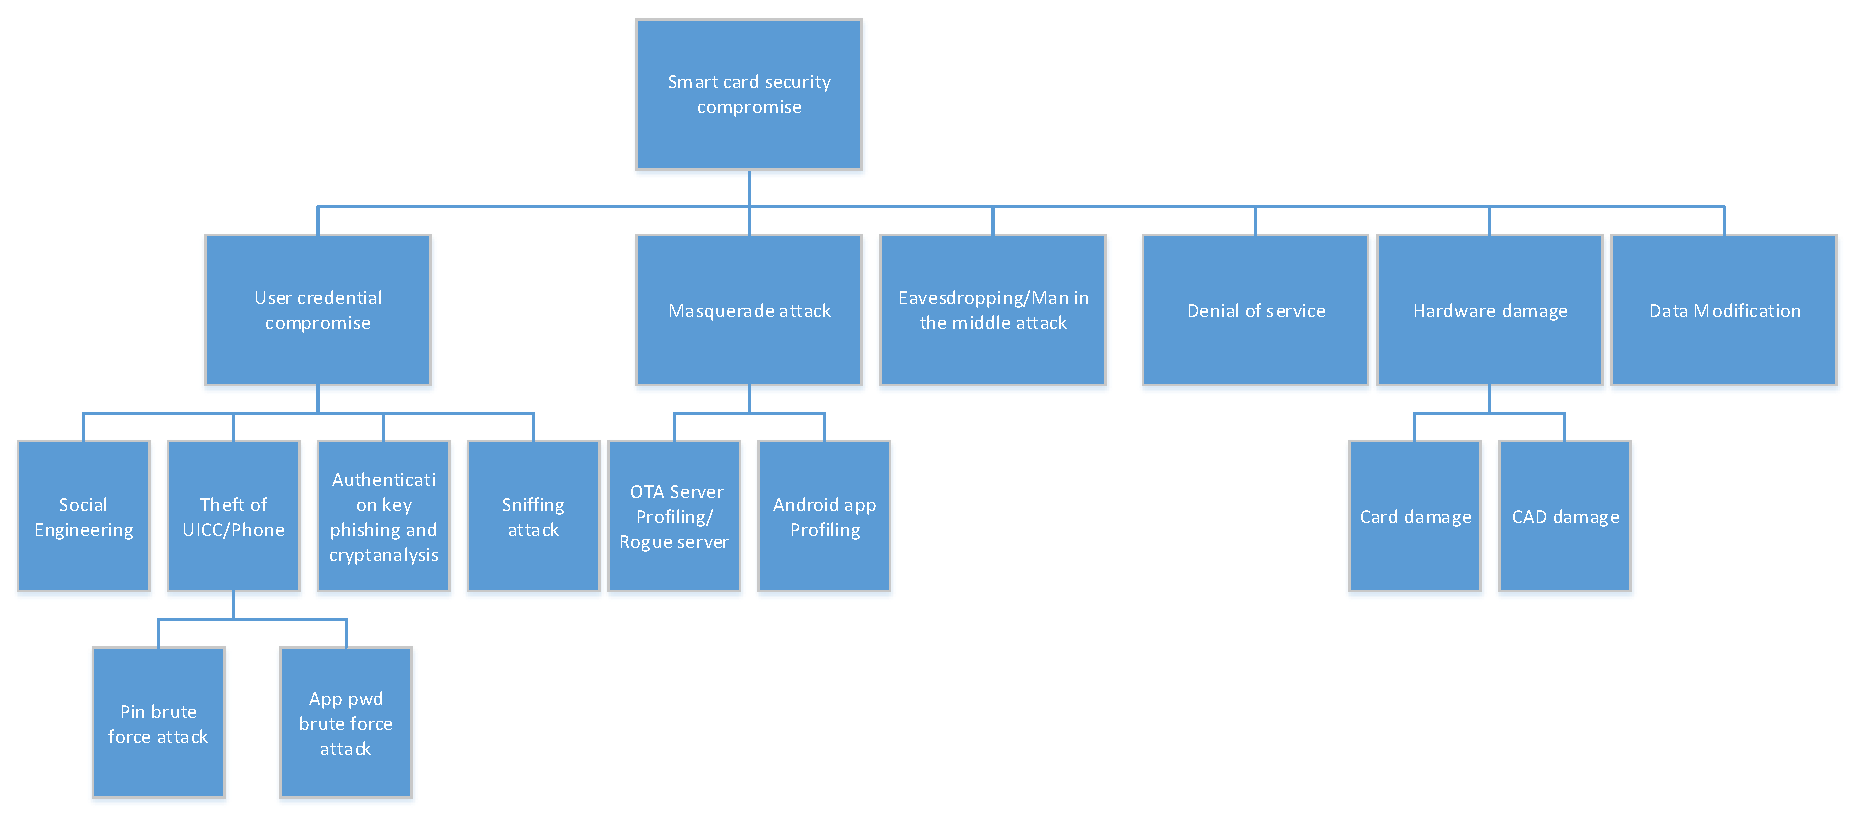
\includegraphics[width=1.2\textwidth]{attack-tree-smartcard}
		\caption{Smartcard Security Compromise}
	\label{fig:attack-tree-smartcard}
\end{figure}
Figure~\ref{fig:attack-tree-smartcard} illustrates the first category of potential threats. Since a number of attacks are listed in the figure which makes it hard to read detailed subcategories, therefore this sub attack tree is also presented as following,

\begin{enumerate}
	\item User credential compromise
  	\begin{enumerate}
    	\item Social Engineering
	\item Theft of UICC/Phone
		\begin{enumerate}
		\item Smart card PIN brute force attack
		\item Android Application password brute force attack
		\end{enumerate}
    	\item Authentication key phishing and cryptanalysis
    	\item  sniffing attack
	\end{enumerate}
	\item Masquerade attack
		\begin{enumerate}
		\item OTA server profiling/Rogue server
		\item Android Application profiling
		\end{enumerate}
	\item Eavesdropping/Man in the middle attack
	\item Denial of service
	\item Hardware damage
		\begin{enumerate}
		\item Card  damage
		\item CAD damage
		\end{enumerate}
	\item  Data Modification
\end{enumerate}

\subsection{Analysis and Countermeasures}
Secure mechanisms and countermeasures against potential threads to the smart card are described as following,
\begin{itemize}
\item \emph{against user credential compromise}. Any security system must have a human as the administrator or user, therefore the secure storage and usage of user credential shows its importance in the realm of computer security. As shown in the attack tree, following potential threads are presented,
\begin{itemize}
\item Social engineering, this attack refers to the process of psychological manipulation of user to for instance give out their password or to believe a fraud. In order to protect the end user, no one can get access to my system, without the UICC smart card and the corresponding user password, which is used to unlock Android  application. In the worst case, which means, user gives his smart phone and password to the attacker, the system is also capable of recording any behaviors taking place during the period of fraud and providing forensic evidence.
\item Theft of Phone or smart card. Even when the attacker manages to steal the smart phone, but without the acknowledge of the PIN and users password, which are used to unlock the smart card and Android Application respectively, he can not get access to the system. Moreover both smart card and my Android Application has the mechanism to block itself after three times of wrong input, which means brute force attack is not an option for the attacker.
\item Key phishing and cryptanalysis/Sniffing. As introduced in ~\ref{labelKeyManagement}, smart card is the secure  credential  storage media and the keys used by smart card consist of various of information, such as key number, key indicator and so on. Consequently, even if the attacker has a segment of credential message, which is captured as a result of key phishing or sniffing, he can never figure out what encryption keys are applied without knowing the smart card key management mechanism and structure.
\end{itemize}
\item \emph{against masquerade attack.} In order to fraud the smart card and to get the credential information stored by it, the attacker could masquerade  himself as either the remote administrator server or the Android Application designed by me.  But any of these two approaches will not work, because the smart card needs to perform TLS secure handshake before exchange any other information with the remote server as standardized by the \emph{GlobalPlatform}. If an Android Application claims himself as the smart card Application, it must provide the according Application signature, as described in essential secure element  control protocols, which are also provided by the \emph{GloabalPlatform}. Since any fraud Application can not pass the exam of providing the correct Application signature, users of smart card will not worry about Android Application masquerade attack. 
\item \emph{against eavesdropping and MitM attacks.} Since the communication between smart card and the remote server is session-based, even when an attacker is able to capture some communication messages, he still can't reply this message to the victims. 
\item \emph{against DoS attack..} The remote administrator server could be a victim of denial of service attack, when the adversary floods message to the server and tries to harm the system. But the remote server applied in my scenario has the message exchanging rate control  mechanism, any partner that floods the message will be banned by the system for a period of time.
\item \emph{against Hardware damage.} Nowadays' smart cards are designed with the protecting mechanisms against physical attacks, such as the already introduced power difference analysis and so on, therefore the major consequence of smart card hardware damage is that, users have to require a new card from the card provider and to bear the inconvenience brought by card damage. 
\item \emph{against data modification.} Data here refers not only to the information stored on the smart card but also the messages exchanged between smart card and the remote server.  As already introduced, smart card is a perfect storage media and independent of other external device. Moreover the exchanged messages are protected from the attacker using  checksum algorithm, which means any information modified by a third party is going to be ignored.
\end{itemize}

\section{Application Level Security Compromise}
In this section, the second category of threads is discussed and accordingly countermeasures are presented.  
\subsection{Sub Attack Tree and its Content}
 \begin{figure}[!htb]
	\centering
	\includegraphics[width=1.2\textwidth]{attack-tree-application}
		\caption{Application Level Security Compromise}
	\label{fig:attack-tree-application}
\end{figure}
The second category of threads which focus on the OPC UA application is figured as ~\ref{fig:attack-tree-application} and  the graph content is described as following,

\begin{enumerate}
	\item Message replay attack
	\item Man in the middle attack
	\item Stealth and Hijacking attack
  	\begin{enumerate}
    	\item Session fixation
	\item Session hijacking
	\end{enumerate}
		
    	\item Request authentication attacks
	\begin{enumerate}
		\item Brute-force attack
		\item Dictionary attacks
		\end{enumerate}
    	\item  sniffing attack - eavesdropping

	\item Data modification
		\begin{enumerate}
		\item Message alternation
		\item Malformed message
		\end{enumerate}
	
	\item Denial of service
		\begin{enumerate}
		\item Well-formed message flooding
		\item Malformed message flooding
		\end{enumerate}

	\item Masquerade attack
		\begin{enumerate}
		\item Server profiling
		\item Rogues server
		\end{enumerate}
\end{enumerate}
\subsection{Analysis and Countermeasures}
In total eight categories of threads, which aim at the OPC UA client and server application code applied in my scenario, are analyzed. They are,

\begin{itemize}
\item \emph{Message replay attack and MitM attack.} Even when an adversary capture a illegal message  exchanged for instance between two housing devices in my scenario, he can never able to reply this message, because each request and response message is protected by its  session IDs, secure channel IDs and alternatively sequence number.
\item \emph{Stealth and Hijacking attack.}In order to perform session hijacking attack, the attacker must firstly compromise the secure channel based on which the session is created. But the employed secure  channel is standardized by Globalplatform and protected with TLS handshake. Therefore, the users don't need to concern attacks in this category.
\item \emph{Request authentication attack.} No matter either the attacker applies brute force attack  or dictionary attack, he only has three password or PIN input chances, which means it is extremely impossible for him to guess the authentication passwords or PIN.
\item \emph{Sniffing.} Encryption algorithms are always  applied in my system, therefore the adversary is not  able to understand  the message he sniffed and the system confidentiality is protected.
\item \emph{Data Modification.} Both  symmetric and asymmetric  signatures are introduced in OPC UA standards, any by third part modified message can not pass the signature examination test and will be ignored.
\item \emph{Denial of service.} In order to protect  the service availability of my system, the message  exchanging rate is controlled. 
\item \emph{Masquerade attack.} Masquerade attacks are impossible in my system for the following reasons. Firstly if a malicious application claims itself to be a OPC UA client or server partner, it must provide necessary secure information such as secure keys and certificates to the other partners before he can perform any other actions. Moreover it also has to be able to perform dual authentication withe the remote administrator server. Even when the fraud application receive a message, it doesn't possess the required  private keys to decrypt the message. 
\end{itemize}

\section{conclusion}
In conclusion, my proposal  system is strong against  the known attacks by adopting the combination of the magic bullet - smart card and the newly released OPC UA specifications. 

\clearemptydoublepage
%######################## Chapter 3 ######################################################
%\clearemptydoublepage
%\input{...}

%######################## Chapter ? ######################################################
%\clearemptydoublepage
\chapter{Summary and Future Work}\label{secSummary}

With the development of M2M and home automatic control technologies, the in this thesis described Smart Home system will be in popular demand in the near future. But since present-day system is frequently exposed in pervasive computing and ubiquitous networking environment, the concept of security is drawing more and more attentions. 

The security feature of smart card as secure token makes this chip sized circuit card the perfect storage media for user credential information. Meanwhile the hardware supports for the execution of encryption algorithms and smart card OS security mechanisms such as key management and secure APDU messaging protocol contribute to add additional secure protection to the system that employs smart card. Moreover by applying well standardized industrial protocols such as RAM/RFM over Http standards from GlobalPlatform and the Simalliance’s OpenMobileAPI, smart card is capable of constructing secure session based connections with remote server and perform dual authentication as well secure messaging with CADs.

The newly released OPC UA specifications provide not only a sophisticated object modelling rules, which can be applied to design domain specific models, but also offer a complex secure policies that have clear security objectives in each lay of system architecture and help to protect OPC UA application from adversary's attacks. 
The in this thesis proposed combination of smart card with OPC UA protocols aims to create a generic communication and connectivity platform for  various vendors manufactured secure devices with strong security supports and consideration. 

In the future, if the study of my proposal goes further, it should be also considered that how to apply the newly proposed LTE technology to benefit the system users with qualified high bandwidth network. Moreover it is also worth thinking, whether it is practical and how to apply Near Field Communication embedded devices in the Smart Home system, for the purpose of providing enhanced secure communication environment, integrating small payment services and etc.

At last, I am grateful for the chance provided by Morpho card Paderborn to write this thesis, especially I want to thank Dr. Simon Oberth\"ur, Dr. Stefan Sauer and Castern Rust, who have given me professional advices for my thesis and help me to finish it.

 


%######################## Remainder ######################################################

%--- bibliography -----------------------------------------------------------------------
%\clearemptydoublepage
%\bibliographystyle{myalphadin}
\bibliographystyle{alphadin}
%\bibliographystyle{alpha}
%\bibliographystyle{geralpha}
%\bibliographystyle{dinat}
%\bibliographystyle{splncs}
\bibliography{myThesis}

%--- index ------------------------------------------------------------------------
%\clearemptydoublepage
%\printindex

\end{document}